\documentclass{article}
\usepackage[utf8]{inputenc}

\usepackage[english]{babel}
\usepackage{amsthm}

\usepackage{amsmath}
\usepackage{amssymb}
\usepackage{amsfonts}
\usepackage{braket}
\usepackage{cancel}

\usepackage{tikz}
\usetikzlibrary{quantikz}

\theoremstyle{definition}
\newtheorem{definition}{Definition}[section]

\usepackage{graphicx}
\graphicspath{ {./} }

\usepackage{biblatex}
\addbibresource{sample.bib}

\usepackage[british]{datetime2}

\usepackage[scr=rsfs]{mathalpha}

\usepackage{csquotes}

\title{Notes}
\author{Emil Sayahi}
\date{\today}

\begin{document}

\maketitle

% \section{Introduction}

% Hello Dr Mirza! This is a test document; here is some \textbf{bold text}, some \emph{italicised text}, and, lastly, an inline equation: $y = mx + b$.

% Below is a table of some $x$ and $y$ values modeled by the following equation:\\
% \[ y = 2x + 1 \]\\

% \begin{tabular}{|l|l|}
%     \hline
%     x & y\\
%     \hline
%     0 & 1\\
%     \hline
%     1 & 3\\
%     \hline
%     2 & 5\\
%     \hline
%     3 & 7\\
%     \hline
%     4 & 9\\
%     \hline
%     5 & 11\\
%     \hline
% \end{tabular}\\

% Here is the Miami University logo:\\

% 
\includegraphics[scale=0.25]{miami-university.png}\\

% Here is one \cite{einstein} citation---and here is a second \cite{dirac} citation.

% \printbibliography

\section{Chapter 1 --- Introduction to Superposition}

\begin{definition}
    \emph{Classical superposition} refers to when two physical quantities are added together to make a new, third one. An example would be constructive or destructive interference with two waves.
\end{definition}
\begin{definition}
    On the quantum scale, objects have properties which can exist in a state of \emph{quantum superposition}. We say that some of their properties, rather than being continuous, can have values inside a set of possible values---such properties are \emph{quantised}. A quantum superposition refers to when a quantised property is not in one discrete state. For example, think of a coin being tossed. The coin, when it lands, can only have two values: heads or tails---this is referred to as having a \emph{definite state}. Until it lands, however, it is both heads and tails simultaneously.
\end{definition}

\section{Chapter 2 --- What Is a Qubit?}

\begin{definition}
    Qubits are the quantum equivalent of classical bits. They can be expressed with \emph{Dirac notation} (eg, $\ket{a}$ refers to a column vector, $a$, while $\bra{b}$ refers to a row vector, $b$).
\end{definition}
\begin{definition}
    Quantum states in a superposition can be expressed as $\alpha \ket{a} + \beta \ket{b}$, where $\alpha$ and $\beta$ are the probability amplitudes for the $\ket{a}$ and $\ket{b}$ states, respectively. The \emph{normalisation rule} is that $\alpha^2 + \beta^2 = 1$; the amplitudes are the square-roots of the probabilities.
\end{definition}

We can express the following quantum state, $\ket{\Psi} = \alpha{\ket{0}} + \beta{\ket{1}}$, with the vector $\ket{\Psi} = \begin{pmatrix}
\alpha\\
\beta
\end{pmatrix}$, where $\ket{0} = \begin{pmatrix}
    1\\
    0
\end{pmatrix}$ and $\ket{1} = \begin{pmatrix}
    0\\
    1
\end{pmatrix}$.

\begin{definition}
    If you multiply a matrix, $A$, by its conjugate transpose, $A^{\dagger}$, and the result is a matrix with $1$s in its main diagonal but $0$s elsewhere (an \emph{identity matrix}), then the original matrix ($A$) is called a \emph{unitary matrix}.
\end{definition}

\begin{definition}
    A \emph{Bloch sphere} can be used to visually represent a quantum state. If an arrow in the sphere is pointing toward one of the poles, it is a definite state. Otherwise, the state is in a superposition.
\end{definition}

\begin{figure}
    \centering
    \begin{tikzpicture}[scale=2]
        % Axes
        \draw[->] (0,0)--(1.2,0) node[right] {$\frac{1}{\sqrt{2}}(\ket{0} + \ket{1})$};
        \draw[->] (0,0)--(0,1.2) node[above] {$\ket{0}$};
        \draw[->] (0,0)--(0,-1.2) node[below] {$\ket{1}$};
        \draw[->] (0,0)--(-1.2,0) node[left] {$\frac{1}{\sqrt{2}}(\ket{0} - \ket{1})$};
        % \draw[->] (0,0)--(-.75,-.5) node[below left] {$x$};
        % Vector and label node
        % \draw[->] (0,0)--(.5,0.866);
        % \draw (.4,.5)  node {${\mathbf v}$};
        \draw (0,0) circle(1);
        \draw[dashed] plot[domain=pi:2*pi] ({cos(\x r)},{.2*sin(\x r)});
        \draw[dashed] plot[domain=0:pi] ({cos(\x r)},{.2*sin(\x r)});
    \end{tikzpicture}
    \caption{A Bloch sphere representation of the quantum state $\ket{\Psi} = \alpha{\ket{0}} + \beta{\ket{1}}$.}\label{fig:ch2fig1}
\end{figure}

\subsection{Single Qubit Gates}
\subsubsection{\emph{X} (`NOT') Gate}
This gate flips a definite state ($\ket{0} \leftrightarrow \ket{1}$); if a qubit is in a superposition, then the superposition also flips.

\begin{figure}[ht]
    \centering
    \begin{quantikz}
        \lstick{$\alpha \ket{0} + \beta \ket{1}$} & \gate{X} & \qw{} \rstick{$\beta \ket{0} + \alpha \ket{1}$}
    \end{quantikz}
    \caption{The probability amplitudes flip.}
\end{figure}

The quantum `NOT' gate can be represented as the following matrix:\\
\[ X = \begin{pmatrix}
    0 & 1\\
    1 & 0
\end{pmatrix} .\]

\subsubsection{Hadamard Gate}
The Hadamard gate takes a qubit in a definite $\ket{0}$ or $\ket{1}$ state, and puts it in a superposition of $\ket{0}$ and $\ket{1}$ states.

\begin{figure}[ht]
    \centering
    \begin{quantikz}
        \lstick{$\ket{0}$} & \gate{H} & \qw{} \rstick{$\frac{1}{\sqrt{2}} (\ket{0} + \ket{1})$}
    \end{quantikz}
    \caption{The initial definite $\ket{0}$ state of the qubit becomes a $\ket{+}$ superposition state.}
\end{figure}

\begin{figure}[ht]
    \centering
    \begin{quantikz}
        \lstick{$\ket{1}$} & \gate{H} & \qw{} \rstick{$\frac{1}{\sqrt{2}} (\ket{0} - \ket{1})$}
    \end{quantikz}
    \caption{The initial definite $\ket{1}$ state of the qubit becomes a $\ket{-}$ superposition state.}
\end{figure}

The Hadamard gate can be represented as the following matrix:\\
\[ H = \frac{1}{\sqrt{2}} \begin{pmatrix}
    1 & 1\\
    1 & -1
\end{pmatrix} .\]

\subsubsection{\emph{Z} Gate}
The $Z$ gate leaves the $\ket{0}$ state unchanged, but flips the sign of the $\ket{1}$ state.

\begin{figure}[ht]
    \centering
    \begin{quantikz}
        \lstick{$\alpha \ket{0} + \beta \ket{1}$} & \gate{Z} & \qw{} \rstick{$\alpha \ket{0} - \beta \ket{1}$}
    \end{quantikz}
    \caption{The state was flipped from a $\ket{+}$ state to a $\ket{-}$ state.}
\end{figure}

The $Z$ gate can be represented as the following matrix:\\
\[ Z = \begin{pmatrix}
    1 & 0\\
    0 & -1
\end{pmatrix} .\]

\begin{figure}[ht]
    \centering
    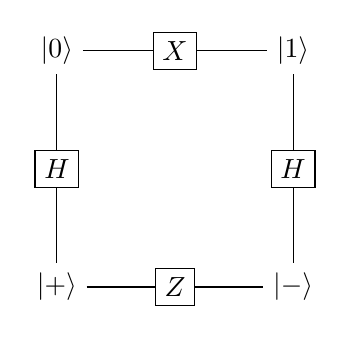
\begin{tikzpicture}[node distance=1.5cm,on grid,auto]
        \node[] (zero)   {$\ket{0}$};
        \node[draw,rectangle,right of=zero] (x)   {$X$};
        \node[right of=x] (one)   {$\ket{1}$};
        \node[draw,rectangle,below of=zero] (h1)   {$H$};
        \node[below of=h1] (plus)   {$\ket{+}$};
        \node[draw,rectangle,right of=plus] (z)   {$Z$};
        \node[draw,rectangle,below of=one] (h2)   {$H$};
        \node[below of=h2] (minus)   {$\ket{-}$};
        \path[shorten >= 0pt, shorten <= 0pt]
            (zero)
                edge node {} (x)
                edge node {} (h1)
            (x)
                edge node {} (one)          
            (one)
                edge node {} (h2)
            (h1)
                edge node {} (plus)
            (plus)
                edge node {} (z)
            (z)
                edge node {} (minus)
            (h2)
                edge node {} (minus);
    \end{tikzpicture}
    \caption{The effects of the $X$, $H$, and $Z$ gates are related.}
\end{figure}

\subsection{Two-Qubit Gates}
\subsubsection{`CNOT' (Controlled `NOT') Gate}
The controlled `NOT' gate is used to entangle two qubits together. The gate takes in a control qubit, a target qubit, and outputs two qubits. The control qubit is untouched, but determines how the target qubit is effected; if the control qubit is $\ket{0}$, then the target qubit is unchanged, but if the control qubit is $\ket{1}$, then the target qubit is flipped ($\ket{0} \leftrightarrow \ket{1}$).

\begin{figure}[ht]
    \centering
    \begin{quantikz}
        \lstick{$\mathrm{Control}\ \ket{A}$} & \ctrl{1} & \qw{} \rstick{$\ket{A}$}\\
        \lstick{$\mathrm{Target}\ \ket{B}$} & \targ{} & \qw{} \rstick{$\ket{A} \oplus \ket{B}$}
    \end{quantikz}
    \caption{A quantum circuit representing the behaviour of the `CNOT' gate.}
\end{figure}

The `CNOT' gate can be represented as the following matrix:\\
\[ \mathrm{CNOT} = \begin{pmatrix}
    1 & 0 & 0 & 0\\
    0 & 1 & 0 & 0\\
    0 & 0 & 0 & 1\\
    0 & 0 & 1 & 0
\end{pmatrix} .\]

\section{Section 2.1 --- Examples of Typical Machine Learning Problems}

\subsection{Image recognition}
A machine learning model can be given images as a matrix of pixels, and tasked with determining what human-recognisable objects are present in the image. In other words, the model can take in a matrix of pixels and determine the appropriate label for the pixel matrix.

\subsection{Time series forecasting}
A machine learning model can be given a series of data points recorded in consecutive time intervals, tasked with the task of forecasting future data points.

\subsection{Hypothesis guessing}
A machine learning model can be given data with some pattern or rules, which the model must determine to predict future elements of the data set. For example, given the vector $\begin{pmatrix}
    4 & 16 & 36 & 100
\end{pmatrix}$, a model could be tasked with completing the pattern until $200$.

\subsection{Board games}
In a context where a machine learning model is preforming actions within an action space, the model is referred to as an \emph{agent}. Often times, an agent can be taught to play a board game using \emph{reinforcement learning}, where the agent is rewarded for preforming positive actions and punished for preforming negative actions, where `negative' and `positive' refer to following pre-determined rules for how to behave, which can include how the action impacts the ultimate outcome---in the case of a board game, whether the action eventually leads to a win, loss, or, if the game allows, a draw. With this style of learning, an agent learns by trial and error.
\begin{definition}
    \emph{Deep learning} is a type of machine learning model, where there are several layers in a `neural network', each layer having at least one `neurone'. All of these artificial neurones are connected to every neurone in the adjacent layers. These neurones have `weights' (a tensor which is updated by training the model), `biases' (a constant term which is updated by training the model), and an `activation function' (which determines if the neurone `fires', or is activated, within the network). With a trained neural network, the input neurons (in the input layer) have their values tensor-multiplied ($\otimes$) with the weights of each connected layer, with the biases of those connected layers added to the resulting tensors. This is done with each successive layer until the output layer, where the values of each output neurone are collected.
\end{definition}

\section{Section 2.2 --- The Three Ingredients of a Learning Problem}
\begin{definition}
    A \emph{supervised learning task} is one in which the data set is labelled, and the task is to predict the appropriate label for a new, unclassified input.
\end{definition}
\begin{definition}
    An \emph{unsupervised learning task} is one in which the data set is not labelled, and the task is to determine the appropriate classes present in the data set, and the elements which belong to each class.
\end{definition}

\subsubsection{Subsection 2.2.1 --- Data}
\begin{definition}
    A machine learning model, in a supervised learning context, attempts to minimise its mistakes; its accuracy can be modelled with another function, called a \emph{loss function}.
\end{definition}
In the context of unsupervised learning, clustering of elements in a data set is done using the distance between the elements.
\begin{definition}
    \emph{Feature selection} refers to the process of determining what variables, predictors, or features are relevant in constructing the appropriate model.
\end{definition}
A data set that has biases within it will result in models that reflect those same biases.
\begin{definition}
    A \emph{classification task} is concerned with labelling data elements with the class that they belong to.
\end{definition}
\begin{definition}
    A \emph{regression task} is concerned with fitting a model to a data set, so that new data elements can be predicted.
\end{definition}

\subsubsection{Subsection 2.2.2 --- Model}
\begin{definition}
    A \emph{model} is something which can be used to approximate observed behaviour. In the context of statistics, data science, and machine learning, a model is a function which attempts to fit the behaviour of a data set.
\end{definition}
\begin{definition}
    A \emph{deterministic model} is a model which provides predictions without a probability attached to it; the model is certain in its predictions, regardless of whether or not the predictions are accurate.
\end{definition}
\begin{definition}
    A \emph{probabilistic model} is a model which is not certain in its predictions, but, instead, has some probability attached with its predictions.
\end{definition}

\subsubsection{Subsection 2.2.3 --- Loss}
\begin{definition}
    We can evaluate the performance of a model by using a \emph{loss function}---a common metric used to define loss is accuracy ($\mathrm{Accuracy} = \frac{\text{Number of correctly classified examples}}{\text{Total number of examples}}$). Regardless of what function we use to define loss, the \emph{error} is the complement of the loss ($\mathrm{Error} = 1 - \mathrm{Loss}$, where $\mathrm{Loss} = \left[0, 1\right)$).
\end{definition}

\section{2.4 --- Training in Unsupervised Learning}
There is no one standard approach to training in unsupervised learning, as the goal of `minimising loss' is difficult to define when we cannot automatically calculate a metric such as accuracy---a model which generates images of zebras, for example, cannot have its imagery automatically evaluated at the end. There are, however, some common approaches, including \emph{generative adversarial
training} and \emph{two-sample testing}.
\begin{definition}
    A \emph{generative adversarial network} is a type of unsupervised learning model, where two models are trained simultaneously: a \emph{generator} and a \emph{discriminator}. The generator attempts to generate data which is similar to the training data, while the discriminator attempts to distinguish between the generated data and the training data. The generator is trained to fool the discriminator, while the discriminator is trained to not be fooled by the generator. Essentially, the generator is trained to generate data which is similar to the training data, while the discriminator is trained to distinguish between the training data and the generated data.
\end{definition}
\begin{definition}
    \emph{Two-sample testing} is a method of unsupervised learning, where the goal is to determine whether two data sets are drawn from the same distribution. This is done by training a model to distinguish between the two data sets, and then evaluating the accuracy of the model.
\end{definition}

\section{Jaynes-Cummings Model}
\begin{definition}
    The number of `\emph{modes}' in a system is the number of different frequencies of electromagnetic radiation in the system. A system where every photon has the same frequency is called \emph{monomodal}, while a system where every photon has a different frequency is called \emph{multimodal}.
\end{definition}

\begin{definition}
    The \emph{Jaynes-Cummings model} is a model which describes the interaction between an atom and some monomodal electromagnetic radiation. When the atom is hit by a photon, it absorbs it and moves to an excited state ($\ket{e}$); when the atom is in an excited state, it can emit a photon and move back to its ground state ($\ket{g}$). The total energy of the system---the \emph{Hamiltonian} of the system---is defined as $\hat{H} = \hat{H}_{\text{atom}} + \hat{H}_{\text{cavity}} + \hat{H}_{\text{interaction}}$.
\end{definition}

\subsubsection{Atom Hamiltonian}
\begin{definition}
    The \emph{atom Hamiltonian} is the Hamiltonian of the atom, which is the sum of the kinetic energy of the atom and the potential energy of the atom.
\end{definition}
\begin{figure}[ht]
    \centering
    \begin{quantikz}
        \lstick[2]{$\Omega = E_{e} - E_{g}$} & \qw{} & \qw{} & \qw{} \rstick{$\ket{0} = \ket{e}$}\\
        \qw{} & \qw{} & \qw{} & \qw{} \rstick{$\ket{1} = \ket{g}$}
    \end{quantikz}
    \caption{The `two-level system' of an atom.}
\end{figure}

The energy of a photon, $E$, can be found with the equation $E = hf$, where $h$ is Planck's constant, and $f$ is the frequency of the photon. It follows from this relation between energy and frequency that the atom Hamiltonian is $\hat{H}_{\text{atom}} = \hbar \Omega \hat{\sigma}_{+}\hat{\sigma}_{-}$, where $\Omega$ is the frequency of the atom, $\hat{\sigma}_{+}$ is the atomic raising operator, and $\hat{\sigma}_{-}$ is the atomic lowering operator.

\begin{definition}
    The \emph{atomic raising operator} is the operator which raises the atom from its ground state to its excited state, and is defined as $\hat{\sigma}_{+} = \ket{e}\bra{g}$. The \emph{atomic lowering operator} is the operator which lowers the atom from its excited state to its ground state, and is defined as $\hat{\sigma}_{-} = \ket{g}\bra{e}$.
\end{definition}

\subsubsection{Electromagnetic Field Hamiltonian}
\begin{definition}
    The \emph{photon creation operator}, $\hat{a}^{+}$, is the operator which creates a photon, defined as $\hat{a}^{+}\ket{n} = \sqrt{n + 1}\ket{n + 1}$. The \emph{photon annihilation operator}, $\hat{a}^{-}$, is the operator which destroys a photon, defined as $\hat{a}^{-}\ket{n} = \sqrt{n}\ket{n-1}$. The \emph{number operator} describes the number of photons in a system, defined as $\hat{a}^{+}\hat{a}^{-}\ket{n} = n\ket{n}$.
\end{definition}

\begin{definition}
    The \emph{electromagnetic field Hamiltonian} is the Hamiltonian of the cavity---the space in which the electromagnetic radiation is contained---defined as $\hat{H}_{\text{cavity}} = \hbar \omega (\hat{a}^{+}\hat{a}^{-})$, where $\omega$ is the frequency of every photon in the cavity (if these frequencies were different, the system would be \emph{multimodal}).
\end{definition}

\subsubsection{Interaction Hamiltonian}
\begin{definition}
    The \emph{light-matter interaction Hamiltonian} is the Hamiltonian which describes the interaction between some monomodal electromagnetic radiation and a single atom, defined as $\hat{H}_{\text{interaction}} = \hbar G (\hat{a}^{+}\hat{\sigma}_{-} + \hat{a}^{-}\hat{\sigma}_{+})$, where $G = \frac{\Omega}{2}$---the strength of the interaction between the atom and the electromagnetic field. $\hat{a}^{+}\hat{\sigma}_{-}$ is the process of the atom emitting a photon, falling to its ground state, while $\hat{a}^{-}\hat{\sigma}_{+}$ is the process of the atom absorbing a photon, rising to its excited state.
\end{definition}

\subsection{Monomodal Single-Photon Problem}
\begin{definition}
    The \emph{Schr{\"o}dinger equation} is the equation which describes how a quantum system changes with time, defined as $i \hbar \frac{\partial \ket{\Psi (t)}}{\partial t} = \hat{H}\ket{\Psi}$, where $\hat{H}$ is the Hamiltonian of the system.
\end{definition}

The state of the system is $\Psi(t) = C_{e}(t)\ket{e}\ket{0} + C_{g}(t)\ket{g}\ket{1}$; inserting the state and Hamiltonian into the Schr{\"o}dinger equation yields $i \hbar \frac{\partial C_{e}(t)}{\partial t}\ket{e}\ket{0} + i \hbar \frac{\partial C_{g}(t)}{\partial t} \ket{g}\ket{1} = (\hbar \Omega \hat{\sigma}_{+}\hat{\sigma}_{-} + \hbar \omega \hat{a}^{+}\hat{a}^{-} + \hbar G(\hat{a}^{+}\hat{\sigma}_{-} + \hat{a}^{-}\hat{\sigma}_{+}))(C_{e}(t)\ket{e}\ket{0} + C_{g}(t)\ket{g}\ket{1})$---$| C_{e}(t) |^{2}$ would be the probability of finding an atom in an excited state, and no photon in the cavity; $| C_{g}(t) |^{2}$ would be the probability of finding an atom in the ground state and one photon in the cavity.

Multiplying the expressions of the prior equation would yield $\hbar \Omega \hat{\sigma}_{+}\hat{\sigma}_{-} C_{e}(t) \ket{e}\ket{0} + \hbar \Omega \hat{\sigma}_{+}\hat{\sigma}_{-} C_{g}(t) \cancelto{0}{\ket{g}}\ket{1} + \hbar \omega \hat{a}^{+}\hat{a}^{-} C_{e}(t) \ket{e}\cancelto{0}{\ket{0}} + \hbar \omega \hat{a}^{+}\hat{a}^{-} C_{g}(t) \ket{g}\ket{1} + \hbar G \hat{a}^{+}\hat{\sigma}_{-} C_{e}(t) \ket{e}\ket{0} + \hbar G \hat{a}^{+}\hat{\sigma}_{-} C_{g}(t) \cancelto{0}{\ket{g}}\cancelto{0}{\ket{1}} + \hbar G \hat{a}^{-}\hat{\sigma}_{+} C_{e}(t) \cancelto{0}{\ket{e}}\cancelto{0}{\ket{0}} + \hbar G \hat{a}^{-}\hat{\sigma}_{+} C_{g}(t) \ket{g}\ket{1} = \hbar \Omega C_{e}(t) \ket{e}\ket{0} + \hbar \omega C_{g}(t) \ket{g}\ket{1} + \hbar G C_{e}(t) \ket{g}\ket{1} + \hbar G C_{g}(t) \ket{e}\ket{0}$, which is to say that $i \hbar \frac{\partial C_{e}(t)}{\partial t}\ket{e}\ket{0} + i \hbar \frac{\partial C_{g}(t)}{\partial t}\ket{g}\ket{1} = \hbar \Omega C_{e}(t) \ket{e}\ket{0} + \hbar \omega C_{g}(t) \ket{g}\ket{1} + \hbar G C_{e}(t) \ket{g}\ket{1} + \hbar G C_{g}(t) \ket{e}\ket{0}$. Projection from the left side by $\bra{e}\bra{0}$ would yield $i \hbar \frac{\partial C_{e}(t)}{\partial t} = \hbar \Omega C_{e}(t) + 0 + 0 + \hbar G C_{g}(t)$, while projection from the left side by $\bra{g}\bra{1}$ would yield $i \hbar \frac{\partial C_{g}(t)}{\partial t} = 0 + \hbar \omega C_{g}(t) + \hbar G C_{e}(t) + 0$.

Next, we calculate the density matricies:
\begin{gather*}
\hat{\rho}_{\text{total}} = \ket{\Psi}\bra{\Psi} = (C_{e}(t)\ket{e; 0} + C_{g}(t)\ket{g; 1})(C_{e}^{*}(t)\bra{e; 0}\\
 + C_{g}^{*}(t)\ket{g; 1}) = C_{e}(t)C_{e}^{*}(t)\ket{e; 0}\bra{e; 0} + C_{e}(t)C_{g}^{*}(t)\ket{e; 0}\bra{g; 1}\\
 + C_{g}(t)C_{e}^{*}(t)\ket{g; 1}\bra{e; 0} + C_{g}(t)C_{g}^{*}(t)\ket{g; 1}\bra{g; 1}\\
\hat{\rho}_{1} = \mathrm{tr}\{ \hat{\rho}_{\text{total}} \} = \braket{0 \mid \hat{\rho}_{\text{total}} \mid 0} + \braket{1 \mid \hat{\rho}_{\text{total}} \mid 1}\\
 = \braket{0 \mid (C_{e}(t)C_{e}^{*}(t)\ket{e; 0}\bra{e; 0} + C_{e}(t)C_{g}^{*}(t)\ket{e; 0}\bra{g; 1} + C_{g}(t)C_{e}^{*}(t)\ket{g; 1}\bra{e; 0} + C_{g}(t)C_{g}^{*}(t)\ket{g; 1}\bra{g; 1}) \mid 0}\\
  + \braket{1 \mid (C_{e}(t)C_{e}^{*}(t)\ket{e; 0}\bra{e; 0} + C_{e}(t)C_{g}^{*}(t)\ket{e; 0}\bra{g; 1} + C_{g}(t)C_{e}^{*}(t)\ket{g; 1}\bra{e; 0} + C_{g}(t)C_{g}^{*}(t)\ket{g; 1}\bra{g; 1}) \mid 1}\\
  = C_{e}(t)C_{e}^{*}(t)\ket{e}\bra{e} + C_{g}(t)C_{g}^{*}(t)\ket{g}\bra{g}
\end{gather*}

\subsection{Monomodal Three-Photon Problem}

The state of the system is $\ket{\Psi(t)} = C_{1}(t) \ket{g_{1}, g_{2}, g_{3}; 3} + C_{2}(t) \ket{e_{1}, g_{2}, g_{3}; 2} + C_{3}(t) \ket{g_{1}, e_{2}, g_{3}; 2} + C_{4}(t) \ket{g_{1}, g_{2}, e_{3}; 2} + C_{5}(t) \ket{e_{1}, e_{2}, g_{3}; 1} + C_{6}(t) \ket{e_{1}, g_{2}, e_{3}; 1} + C_{7}(t) \ket{g_{1}, e_{2}, e_{3}; 1} + C_{8}(t) \ket{e_{1}, e_{2}, e_{3}; 0}$.

The Hamiltonian of the system is $\hat{H} = \sum_{i = 1}^{3} \hbar \Omega_{i} \hat{\sigma}_{i+}\hat{\sigma}_{i-} + \hbar \omega \hat{a}^{+}\hat{a}^{-} + \sum_{i = 1}^{3} \hbar G_{i} (\hat{a}^{+}\hat{\sigma}_{i-} + \hat{a}^{-}\hat{\sigma}_{i+})$, where $\Omega_{i}$ is the frequency of the $i$th atom, $\omega$ is the frequency of the photons in the system, $\hat{\sigma}_{i+}$ is the atomic raising operator of the $i$th atom, $\hat{\sigma}_{i-}$ is the atomic lowering operator of the $i$th atom, $\hat{a}^{+}$ is the photon creation operator of every photon, $\hat{a}^{-}$ is the photon annihilation operator of every photon, and $G_{i}$ is the strength of the interaction between the $i$th atom and the photons.

Inserting the state and Hamiltonian into the Schr{\"o}dinger equation yields $i \hbar \frac{\partial C_{1}(t)}{\partial t} \ket{g_{1}, g_{2}, g_{3}; 3} + i \hbar \frac{\partial C_{2}(t)}{\partial t} \ket{e_{1}, g_{2}, g_{3}; 2} + i \hbar \frac{\partial C_{3}(t)}{\partial t} \ket{g_{1}, e_{2}, g_{3}; 2} + i \hbar \frac{\partial C_{4}(t)}{\partial t} \ket{g_{1}, g_{2}, e_{3}; 2} + i \hbar \frac{\partial C_{5}(t)}{\partial t} \ket{e_{1}, e_{2}, g_{3}; 1} + i \hbar \frac{\partial C_{6}(t)}{\partial t} \ket{e_{1}, g_{2}, e_{3}; 1} + i \hbar \frac{\partial C_{7}(t)}{\partial t} \ket{g_{1}, e_{2}, e_{3}; 1} + i \hbar \frac{\partial C_{8}(t)}{\partial t} \ket{e_{1}, e_{2}, e_{3}; 0} = (\hbar \Omega_{1} \hat{\sigma}_{1+}\hat{\sigma}_{1-} + \hbar \Omega_{2} \hat{\sigma}_{2+}\hat{\sigma}_{2-} + \hbar \Omega_{3} \hat{\sigma}_{3+}\hat{\sigma}_{3-} + \hbar \omega \hat{a}^{+}\hat{a}^{-} + \hbar G_{1} (\hat{a}^{+}\hat{\sigma}_{1-} + \hat{a}^{-}\hat{\sigma}_{1+}) + \hbar G_{2} (\hat{a}^{+}\hat{\sigma}_{2-} + \hat{a}^{-}\hat{\sigma}_{2+}) + \hbar G_{3} (\hat{a}^{+}\hat{\sigma}_{3-} + \hat{a}^{-}\hat{\sigma}_{3+}))(C_{1}(t) \ket{g_{1}, g_{2}, g_{3}; 3} + C_{2}(t) \ket{e_{1}, g_{2}, g_{3}; 2} + C_{3}(t) \ket{g_{1}, e_{2}, g_{3}; 2} + C_{4}(t) \ket{g_{1}, g_{2}, e_{3}; 2} + C_{5}(t) \ket{e_{1}, e_{2}, g_{3}; 1} + C_{6}(t) \ket{e_{1}, g_{2}, e_{3}; 1} + C_{7}(t) \ket{g_{1}, e_{2}, e_{3}; 1} + C_{8}(t) \ket{e_{1}, e_{2}, e_{3}; 0})$.\\

We begin multiplying the expressions of the prior equation:\\
\begin{enumerate}
    \item $(\hbar \Omega_{1} \hat{\sigma}_{1+}\hat{\sigma}_{1-})(\Psi(t)) = \hbar \Omega_{1} \hat{\sigma}_{1+}\hat{\sigma}_{1-} C_{1}(t) \ket{\cancelto{0}{g_{1}}, g_{2}, g_{3}; 3} + \hbar \Omega_{1} \hat{\sigma}_{1+}\hat{\sigma}_{1-} C_{2}(t) \ket{e_{1}, g_{2}, g_{3}; 2} + \hbar \Omega_{1} \hat{\sigma}_{1+}\hat{\sigma}_{1-} C_{3}(t) \ket{\cancelto{0}{g_{1}}, e_{2}, g_{3}; 2} + \hbar \Omega_{1} \hat{\sigma}_{1+}\hat{\sigma}_{1-} C_{4}(t) \ket{\cancelto{0}{g_{1}}, g_{2}, e_{3}; 2} + \hbar \Omega_{1} \hat{\sigma}_{1+}\hat{\sigma}_{1-} C_{5}(t) \ket{e_{1}, e_{2}, g_{3}; 1} + \hbar \Omega_{1} \hat{\sigma}_{1+}\hat{\sigma}_{1-} C_{6}(t) \ket{e_{1}, g_{2}, e_{3}; 1} + \hbar \Omega_{1} \hat{\sigma}_{1+}\hat{\sigma}_{1-} C_{7}(t) \ket{\cancelto{0}{g_{1}}, e_{2}, e_{3}; 1} + \hbar \Omega_{1} \hat{\sigma}_{1+}\hat{\sigma}_{1-} C_{8}(t) \ket{e_{1}, e_{2}, e_{3}; 0} = \hbar \Omega_{1}C_{2}(t)\ket{e_{1}, g_{2}, g_{3}; 2} + \hbar \Omega_{1}C_{5}(t)\ket{e_{1}, e_{2}, g_{3}; 1} + \hbar \Omega_{1}C_{6}(t)\ket{e_{1}, g_{2}, e_{3}; 1} + \hbar \Omega_{1}C_{8}(t)\ket{e_{1}, e_{2}, e_{3}; 0}$
    \item $(\hbar \Omega_{2} \hat{\sigma}_{2+}\hat{\sigma}_{2-})(\Psi(t)) = \hbar \Omega_{2} \hat{\sigma}_{2+}\hat{\sigma}_{2-}C_{1}(t) \ket{g_{1}, \cancelto{0}{g_{2}}, g_{3}; 3} + \hbar \Omega_{2} \hat{\sigma}_{2+}\hat{\sigma}_{2-}C_{2}(t) \ket{e_{1}, \cancelto{0}{g_{2}}, g_{3}; 2} + \hbar \Omega_{2} \hat{\sigma}_{2+}\hat{\sigma}_{2-}C_{3}(t) \ket{g_{1}, e_{2}, g_{3}; 2} + \hbar \Omega_{2} \hat{\sigma}_{2+}\hat{\sigma}_{2-}C_{4}(t) \ket{g_{1}, \cancelto{0}{g_{2}}, e_{3}; 2} + \hbar \Omega_{2} \hat{\sigma}_{2+}\hat{\sigma}_{2-}C_{5}(t) \ket{e_{1}, e_{2}, g_{3}; 1} + \hbar \Omega_{2} \hat{\sigma}_{2+}\hat{\sigma}_{2-}C_{6}(t) \ket{e_{1}, \cancelto{0}{g_{2}}, e_{3}; 1} + \hbar \Omega_{2} \hat{\sigma}_{2+}\hat{\sigma}_{2-}C_{7}(t) \ket{g_{1}, e_{2}, e_{3}; 1} + \hbar \Omega_{2} \hat{\sigma}_{2+}\hat{\sigma}_{2-}C_{8}(t) \ket{e_{1}, e_{2}, e_{3}; 0} = \hbar \Omega_{2} C_{3}(t)\ket{g_{1}, e_{2}, g_{3}; 2} + \hbar \Omega_{2} C_{5}(t)\ket{e_{1}, e_{2}, g_{3}; 1} + \hbar \Omega_{2} C_{7}(t)\ket{g_{1}, e_{2}, e_{3}; 1} + \hbar \Omega_{2} C_{8}(t)\ket{e_{1}, e_{2}, e_{3}; 0}$
    \item $(\hbar \Omega_{3} \hat{\sigma}_{3+}\hat{\sigma}_{3-})(\Psi(t)) = \hbar \Omega_{3} \hat{\sigma}_{3+}\hat{\sigma}_{3-}C_{1}(t) \ket{g_{1}, g_{2}, \cancelto{0}{g_{3}}; 3} + \hbar \Omega_{3} \hat{\sigma}_{3+}\hat{\sigma}_{3-}C_{2}(t) \ket{e_{1}, g_{2}, \cancelto{0}{g_{3}}; 2} + \hbar \Omega_{3} \hat{\sigma}_{3+}\hat{\sigma}_{3-}C_{3}(t) \ket{g_{1}, e_{2}, \cancelto{0}{g_{3}}; 2} + \hbar \Omega_{3} \hat{\sigma}_{3+}\hat{\sigma}_{3-}C_{4}(t) \ket{g_{1}, g_{2}, e_{3}; 2} + \hbar \Omega_{3} \hat{\sigma}_{3+}\hat{\sigma}_{3-}C_{5}(t) \ket{e_{1}, e_{2}, \cancelto{0}{g_{3}}; 1} + \hbar \Omega_{3} \hat{\sigma}_{3+}\hat{\sigma}_{3-}C_{6}(t) \ket{e_{1}, g_{2}, e_{3}; 1} + \hbar \Omega_{3} \hat{\sigma}_{3+}\hat{\sigma}_{3-}C_{7}(t) \ket{g_{1}, e_{2}, e_{3}; 1} + \hbar \Omega_{3} \hat{\sigma}_{3+}\hat{\sigma}_{3-}C_{8}(t) \ket{e_{1}, e_{2}, e_{3}; 0} = \hbar \Omega_{3} C_{4}(t)\ket{g_{1}, g_{2}, e_{3}; 2} + \hbar \Omega_{3} C_{6}(t)\ket{e_{1}, g_{2}, e_{3}; 1} + \hbar \Omega_{3} C_{7}(t)\ket{g_{1}, e_{2}, e_{3}; 1} + \hbar \Omega_{3} C_{8}(t)\ket{e_{1}, e_{2}, e_{3}; 0}$
    \item $(\hbar \omega \hat{a}^{+}\hat{a}^{-})(\Psi(t)) = \hbar \omega \hat{a}^{+}\hat{a}^{-}C_{1}(t) \ket{g_{1}, g_{2}, g_{3}; 3} + \hbar \omega \hat{a}^{+}\hat{a}^{-}C_{2}(t) \ket{e_{1}, g_{2}, g_{3}; 2} + \hbar \omega \hat{a}^{+}\hat{a}^{-}C_{3}(t) \ket{g_{1}, e_{2}, g_{3}; 2} + \hbar \omega \hat{a}^{+}\hat{a}^{-}C_{4}(t) \ket{g_{1}, g_{2}, e_{3}; 2} + \hbar \omega \hat{a}^{+}\hat{a}^{-}C_{5}(t) \ket{e_{1}, e_{2}, g_{3}; 1} + \hbar \omega \hat{a}^{+}\hat{a}^{-}C_{6}(t) \ket{e_{1}, g_{2}, e_{3}; 1} + \hbar \omega \hat{a}^{+}\hat{a}^{-}C_{7}(t) \ket{g_{1}, e_{2}, e_{3}; 1} + \hbar \omega \hat{a}^{+}\hat{a}^{-}C_{8}(t) \ket{e_{1}, e_{2}, e_{3}; \cancelto{0}{0}} = 3 \hbar \omega C_{1}(t) \ket{g_{1}, g_{2}, g_{3}; 3} + 2 \hbar \omega C_{2}(t) \ket{e_{1}, g_{2}, g_{3}; 2} + 2 \hbar \omega C_{3}(t) \ket{g_{1}, e_{2}, g_{3}; 2} + 2 \hbar \omega C_{4}(t) \ket{g_{1}, g_{2}, e_{3}; 2} + \hbar \omega C_{5}(t) \ket{e_{1}, e_{2}, g_{3}; 1} + \hbar \omega C_{6}(t) \ket{e_{1}, g_{2}, e_{3}; 1} + \hbar \omega C_{7}(t) \ket{g_{1}, e_{2}, e_{3}; 1}$
    \item $(\hbar G_{1} (\hat{a}^{+}\hat{\sigma}_{1-} + \hat{a}^{-}\hat{\sigma}_{1+}))(\Psi(t)) = \hbar G_{1}\hat{a}^{+}\hat{\sigma}_{1-}C_{1}(t) \ket{\cancelto{0}{g_{1}}, g_{2}, g_{3}; \cancelto{0}{3}} + \hbar G_{1}\hat{a}^{+}\hat{\sigma}_{1-}C_{2}(t) \ket{\cancelto{g_{1}}{e_{1}}, g_{2}, g_{3}; \cancelto{3}{2}} + \hbar G_{1}\hat{a}^{+}\hat{\sigma}_{1-}C_{3}(t) \ket{\cancelto{0}{g_{1}}, e_{2}, g_{3}; \cancelto{3}{2}} + \hbar G_{1}\hat{a}^{+}\hat{\sigma}_{1-}C_{4}(t) \ket{\cancelto{0}{g_{1}}, g_{2}, e_{3}; \cancelto{3}{2}} + \hbar G_{1}\hat{a}^{+}\hat{\sigma}_{1-}C_{5}(t) \ket{\cancelto{g_{1}}{e_{1}}, e_{2}, g_{3}; \cancelto{2}{1}} + \hbar G_{1}\hat{a}^{+}\hat{\sigma}_{1-}C_{6}(t) \ket{\cancelto{g_{1}}{e_{1}}, g_{2}, e_{3}; \cancelto{2}{1}} + \hbar G_{1}\hat{a}^{+}\hat{\sigma}_{1-}C_{7}(t) \ket{\cancelto{0}{g_{1}}, e_{2}, e_{3}; \cancelto{2}{1}} + \hbar G_{1}\hat{a}^{+}\hat{\sigma}_{1-}C_{8}(t) \ket{\cancelto{g_{1}}{e_{1}}, e_{2}, e_{3}; \cancelto{1}{0}} + \hbar G_{1}\hat{a}^{-}\hat{\sigma}_{1+}C_{1}(t) \ket{\cancelto{e_{1}}{g_{1}}, g_{2}, g_{3}; \cancelto{2}{3}} + \hbar G_{1}\hat{a}^{-}\hat{\sigma}_{1+}C_{2}(t) \ket{\cancelto{0}{e_{1}}, g_{2}, g_{3}; \cancelto{1}{2}} + \hbar G_{1}\hat{a}^{-}\hat{\sigma}_{1+}C_{3}(t) \ket{\cancelto{e_{1}}{g_{1}}, e_{2}, g_{3}; \cancelto{1}{2}} + \hbar G_{1}\hat{a}^{-}\hat{\sigma}_{1+}C_{4}(t) \ket{\cancelto{e_{1}}{g_{1}}, g_{2}, e_{3}; \cancelto{1}{2}} + \hbar G_{1}\hat{a}^{-}\hat{\sigma}_{1+}C_{5}(t) \ket{\cancelto{0}{e_{1}}, e_{2}, g_{3}; \cancelto{0}{1}} + \hbar G_{1}\hat{a}^{-}\hat{\sigma}_{1+}C_{6}(t) \ket{\cancelto{0}{e_{1}}, g_{2}, e_{3}; \cancelto{0}{1}} + \hbar G_{1}\hat{a}^{-}\hat{\sigma}_{1+}C_{7}(t) \ket{\cancelto{e_{1}}{g_{1}}, e_{2}, e_{3}; \cancelto{0}{1}} + \hbar G_{1}\hat{a}^{-}\hat{\sigma}_{1+}C_{8}(t) \ket{\cancelto{0}{e_{1}}, e_{2}, e_{3}; \cancelto{0}{0}} = \sqrt{3} \hbar G_{1}C_{2}(t)\ket{g_{1}, g_{2}, g_{3}; 3} + \sqrt{2} \hbar G_{1}C_{5}(t)\ket{g_{1}, e_{2}, g_{3}; 2} + \sqrt{2} \hbar G_{1}C_{6}(t)\ket{g_{1}, g_{2}, e_{3}; 2} + \hbar G_{1}C_{8}\ket{g_{1}, e_{2}, e_{3}; 1} + \sqrt{3} \hbar G_{1}C_{1}(t)\ket{e_{1}, g_{2}, g_{3}; 2} + \sqrt{2} \hbar G_{1}C_{3}(t)\ket{e_{1}, e_{2}, g_{3}; 1} + \sqrt{2} \hbar G_{1}C_{4}(t)\ket{e_{1}, g_{2}, e_{3}; 1} + \hbar G_{1}C_{7}(t)\ket{e_{1}, e_{2}, e_{3}; 0}$
    \item $(\hbar G_{2} (\hat{a}^{+}\hat{\sigma}_{2-} + \hat{a}^{-}\hat{\sigma}_{2+}))(\Psi(t)) = \hbar G_{2}\hat{a}^{+}\hat{\sigma}_{2-}C_{1}(t) \ket{g_{1}, \cancelto{0}{g_{2}}, g_{3}; \cancelto{0}{3}} + \hbar G_{2}\hat{a}^{+}\hat{\sigma}_{2-}C_{2}(t) \ket{e_{1}, \cancelto{0}{g_{2}}, g_{3}; \cancelto{3}{2}} + \hbar G_{2}\hat{a}^{+}\hat{\sigma}_{2-}C_{3}(t) \ket{g_{1}, \cancelto{g_{2}}{e_{2}}, g_{3}; \cancelto{3}{2}} + \hbar G_{2}\hat{a}^{+}\hat{\sigma}_{2-}C_{4}(t) \ket{g_{1}, \cancelto{0}{g_{2}}, e_{3}; \cancelto{3}{2}} + \hbar G_{2}\hat{a}^{+}\hat{\sigma}_{2-}C_{5}(t) \ket{e_{1}, \cancelto{g_{2}}{e_{2}}, g_{3}; \cancelto{2}{1}} + \hbar G_{2}\hat{a}^{+}\hat{\sigma}_{2-}C_{6}(t) \ket{e_{1}, \cancelto{0}{g_{2}}, e_{3}; \cancelto{2}{1}} + \hbar G_{2}\hat{a}^{+}\hat{\sigma}_{2-}C_{7}(t) \ket{g_{1}, \cancelto{g_{2}}{e_{2}}, e_{3}; \cancelto{2}{1}} + \hbar G_{2}\hat{a}^{+}\hat{\sigma}_{2-}C_{8}(t) \ket{e_{1}, \cancelto{g_{2}}{e_{2}}, e_{3}; \cancelto{1}{0}} + \hbar G_{2}\hat{a}^{-}\hat{\sigma}_{2+}C_{1}(t) \ket{g_{1}, \cancelto{e_{2}}{g_{2}}, g_{3}; \cancelto{2}{3}} + \hbar G_{2}\hat{a}^{-}\hat{\sigma}_{2+}C_{2}(t) \ket{e_{1}, \cancelto{e_{2}}{g_{2}}, g_{3}; \cancelto{1}{2}} + \hbar G_{2}\hat{a}^{-}\hat{\sigma}_{2+}C_{3}(t) \ket{g_{1}, \cancelto{0}{e_{2}}, g_{3}; \cancelto{1}{2}} + \hbar G_{2}\hat{a}^{-}\hat{\sigma}_{2+}C_{4}(t) \ket{g_{1}, \cancelto{e_{2}}{g_{2}}, e_{3}; \cancelto{1}{2}} + \hbar G_{2}\hat{a}^{-}\hat{\sigma}_{2+}C_{5}(t) \ket{e_{1}, \cancelto{0}{e_{2}}, g_{3}; \cancelto{0}{1}} + \hbar G_{2}\hat{a}^{-}\hat{\sigma}_{2+}C_{6}(t) \ket{e_{1}, \cancelto{e_{2}}{g_{2}}, e_{3}; \cancelto{0}{1}} + \hbar G_{2}\hat{a}^{-}\hat{\sigma}_{2+}C_{7}(t) \ket{g_{1}, \cancelto{0}{e_{2}}, e_{3}; \cancelto{0}{1}} + \hbar G_{2}\hat{a}^{-}\hat{\sigma}_{2+}C_{8}(t) \ket{e_{1}, \cancelto{0}{e_{2}}, e_{3}; \cancelto{0}{0}} = \sqrt{3} \hbar G_{2}C_{3}(t)\ket{g_{1}, g_{2}, g_{3}; 3} + \sqrt{2} \hbar G_{2}C_{5}(t)\ket{e_{1}, g_{2}, g_{3}; 2} + \sqrt{2} \hbar G_{2}C_{7}(t)\ket{g_{1}, g_{2}, e_{3}; 2} + \hbar G_{2}C_{8}(t)\ket{e_{1}, g_{2}, e_{3}; 1} + \sqrt{3} \hbar G_{2}C_{1}(t)\ket{g_{1}, e_{2}, g_{3}; 2} + \sqrt{2} \hbar G_{2}C_{2}(t)\ket{e_{1}, e_{2}, g_{3}; 1} + \sqrt{2} \hbar G_{2}C_{4}(t)\ket{g_{1}, e_{2}, e_{3}; 1} + \hbar G_{2}C_{6}(t)\ket{e_{1}, e_{2}, e_{3}; 0}$
    \item $(\hbar G_{3} (\hat{a}^{+}\hat{\sigma}_{3-} + \hat{a}^{-}\hat{\sigma}_{3+}))(\Psi(t)) = \hbar G_{3}\hat{a}^{+}\hat{\sigma}_{3-}C_{1}(t) \ket{g_{1}, g_{2}, \cancelto{0}{g_{3}}; \cancelto{0}{3}} + \hbar G_{3}\hat{a}^{+}\hat{\sigma}_{3-}C_{2}(t) \ket{e_{1}, g_{2}, \cancelto{0}{g_{3}}; \cancelto{3}{2}} + \hbar G_{3}\hat{a}^{+}\hat{\sigma}_{3-}C_{3}(t) \ket{g_{1}, e_{2}, \cancelto{0}{g_{3}}; \cancelto{3}{2}} + \hbar G_{3}\hat{a}^{+}\hat{\sigma}_{3-}C_{4}(t) \ket{g_{1}, g_{2}, \cancelto{g_{3}}{e_{3}}; \cancelto{3}{2}} + \hbar G_{3}\hat{a}^{+}\hat{\sigma}_{3-}C_{5}(t) \ket{e_{1}, e_{2}, \cancelto{0}{g_{3}}; \cancelto{2}{1}} + \hbar G_{3}\hat{a}^{+}\hat{\sigma}_{3-}C_{6}(t) \ket{e_{1}, g_{2}, \cancelto{g_{3}}{e_{3}}; \cancelto{2}{1}} + \hbar G_{3}\hat{a}^{+}\hat{\sigma}_{3-}C_{7}(t) \ket{g_{1}, e_{2}, \cancelto{g_{3}}{e_{3}}; \cancelto{2}{1}} + \hbar G_{3}\hat{a}^{+}\hat{\sigma}_{3-}C_{8}(t) \ket{e_{1}, e_{2}, \cancelto{g_{3}}{e_{3}}; \cancelto{1}{0}} + \hbar G_{3}\hat{a}^{-}\hat{\sigma}_{3+}C_{1}(t) \ket{g_{1}, g_{2}, \cancelto{e_{3}}{g_{3}}; \cancelto{2}{3}} + \hbar G_{3}\hat{a}^{-}\hat{\sigma}_{3+}C_{2}(t) \ket{e_{1}, g_{2}, \cancelto{e_{3}}{g_{3}}; \cancelto{1}{2}} + \hbar G_{3}\hat{a}^{-}\hat{\sigma}_{3+}C_{3}(t) \ket{g_{1}, e_{2}, \cancelto{e_{3}}{g_{3}}; \cancelto{1}{2}} + \hbar G_{3}\hat{a}^{-}\hat{\sigma}_{3+}C_{4}(t) \ket{g_{1}, g_{2}, \cancelto{0}{e_{3}}; \cancelto{1}{2}} + \hbar G_{3}\hat{a}^{-}\hat{\sigma}_{3+}C_{5}(t) \ket{e_{1}, e_{2}, \cancelto{e_{3}}{g_{3}}; \cancelto{0}{1}} + \hbar G_{3}\hat{a}^{-}\hat{\sigma}_{3+}C_{6}(t) \ket{e_{1}, g_{2}, \cancelto{0}{e_{3}}; \cancelto{0}{1}} + \hbar G_{3}\hat{a}^{-}\hat{\sigma}_{3+}C_{7}(t) \ket{g_{1}, e_{2}, \cancelto{0}{e_{3}}; \cancelto{0}{1}} + \hbar G_{3}\hat{a}^{-}\hat{\sigma}_{3+}C_{8}(t) \ket{e_{1}, e_{2}, \cancelto{0}{e_{3}}; \cancelto{0}{0}} = \sqrt{3} \hbar G_{3}C_{4}(t)\ket{g_{1}, g_{2}, g_{3}; 3} + \sqrt{2} \hbar G_{3}C_{6}(t)\ket{e_{1}, g_{2}, g_{3}; 2} + \sqrt{2} \hbar G_{3}C_{7}(t)\ket{g_{1}, e_{2}, g_{3}; 2} + \hbar G_{3}C_{8}(t)\ket{e_{1}, e_{2}, g_{3}; 1} + \sqrt{3} \hbar G_{3}C_{1}(t)\ket{g_{1}, g_{2}, e_{3}; 2} + \sqrt{2} \hbar G_{3}C_{2}(t)\ket{e_{1}, g_{2}, e_{3}; 1} + \sqrt{2} \hbar G_{3}C_{3}(t)\ket{g_{1}, e_{2}, e_{3}; 1} + \hbar G_{3}C_{5}(t)\ket{e_{1}, e_{2}, e_{3}; 0}$.
\end{enumerate}

This yields:\\

$i \hbar \frac{\partial C_{1}(t)}{\partial t} \ket{g_{1}, g_{2}, g_{3}; 3} + i \hbar \frac{\partial C_{2}(t)}{\partial t} \ket{e_{1}, g_{2}, g_{3}; 2} + i \hbar \frac{\partial C_{3}(t)}{\partial t} \ket{g_{1}, e_{2}, g_{3}; 2} + i \hbar \frac{\partial C_{4}(t)}{\partial t} \ket{g_{1}, g_{2}, e_{3}; 2} + i \hbar \frac{\partial C_{5}(t)}{\partial t} \ket{e_{1}, e_{2}, g_{3}; 1} + i \hbar \frac{\partial C_{6}(t)}{\partial t} \ket{e_{1}, g_{2}, e_{3}; 1} + i \hbar \frac{\partial C_{7}(t)}{\partial t} \ket{g_{1}, e_{2}, e_{3}; 1} + i \hbar \frac{\partial C_{8}(t)}{\partial t} \ket{e_{1}, e_{2}, e_{3}; 0} = \hbar \Omega_{1}C_{2}(t)\ket{e_{1}, g_{2}, g_{3}; 2} + \hbar \Omega_{1}C_{5}(t)\ket{e_{1}, e_{2}, g_{3}; 1} + \hbar \Omega_{1}C_{6}(t)\ket{e_{1}, g_{2}, e_{3}; 1} + \hbar \Omega_{1}C_{8}(t)\ket{e_{1}, e_{2}, e_{3}; 0} + \hbar \Omega_{3} C_{4}(t)\ket{g_{1}, g_{2}, e_{3}; 2} + \hbar \Omega_{3} C_{6}(t)\ket{e_{1}, g_{2}, e_{3}; 1} + \hbar \Omega_{3} C_{7}(t)\ket{g_{1}, e_{2}, e_{3}; 1} + \hbar \Omega_{3} C_{8}(t)\ket{e_{1}, e_{2}, e_{3}; 0} + 3 \hbar \omega C_{1}(t) \ket{g_{1}, g_{2}, g_{3}; 3} + 2 \hbar \omega C_{2}(t) \ket{e_{1}, g_{2}, g_{3}; 2} + 2 \hbar \omega C_{3}(t) \ket{g_{1}, e_{2}, g_{3}; 2} + 2 \hbar \omega C_{4}(t) \ket{g_{1}, g_{2}, e_{3}; 2} + \hbar \omega C_{5}(t) \ket{e_{1}, e_{2}, g_{3}; 1} + \hbar \omega C_{6}(t) \ket{e_{1}, g_{2}, e_{3}; 1} + \hbar \omega C_{7}(t) \ket{g_{1}, e_{2}, e_{3}; 1} + \sqrt{3} \hbar G_{1}C_{2}(t)\ket{g_{1}, g_{2}, g_{3}; 3} + \sqrt{2} \hbar G_{1}C_{5}(t)\ket{g_{1}, e_{2}, g_{3}; 2} + \sqrt{2} \hbar G_{1}C_{6}(t)\ket{g_{1}, g_{2}, e_{3}; 2} + \hbar G_{1}C_{8}\ket{g_{1}, e_{2}, e_{3}; 1} + \sqrt{3} \hbar G_{1}C_{1}(t)\ket{e_{1}, g_{2}, g_{3}; 2} + \sqrt{2} \hbar G_{1}C_{3}(t)\ket{e_{1}, e_{2}, g_{3}; 1} + \sqrt{2} \hbar G_{1}C_{4}(t)\ket{e_{1}, g_{2}, e_{3}; 1} + \hbar G_{1}C_{7}(t)\ket{e_{1}, e_{2}, e_{3}; 0} + \sqrt{3} \hbar G_{2}C_{3}(t)\ket{g_{1}, g_{2}, g_{3}; 3} + \sqrt{2} \hbar G_{2}C_{5}(t)\ket{e_{1}, g_{2}, g_{3}; 2} + \sqrt{2} \hbar G_{2}C_{7}(t)\ket{g_{1}, g_{2}, e_{3}; 2} + \hbar G_{2}C_{8}(t)\ket{e_{1}, g_{2}, e_{3}; 1} + \sqrt{3} \hbar G_{2}C_{1}(t)\ket{g_{1}, e_{2}, g_{3}; 2} + \sqrt{2} \hbar G_{2}C_{2}(t)\ket{e_{1}, e_{2}, g_{3}; 1} + \sqrt{2} \hbar G_{2}C_{4}(t)\ket{g_{1}, e_{2}, e_{3}; 1} + \hbar G_{2}C_{6}(t)\ket{e_{1}, e_{2}, e_{3}; 0} + \sqrt{3} \hbar G_{3}C_{4}(t)\ket{g_{1}, g_{2}, g_{3}; 3} + \sqrt{2} \hbar G_{3}C_{6}(t)\ket{e_{1}, g_{2}, g_{3}; 2} + \sqrt{2} \hbar G_{3}C_{7}(t)\ket{g_{1}, e_{2}, g_{3}; 2} + \hbar G_{3}C_{8}(t)\ket{e_{1}, e_{2}, g_{3}; 1} + \sqrt{3} \hbar G_{3}C_{1}(t)\ket{g_{1}, g_{2}, e_{3}; 2} + \sqrt{2} \hbar G_{3}C_{2}(t)\ket{e_{1}, g_{2}, e_{3}; 1} + \sqrt{2} \hbar G_{3}C_{3}(t)\ket{g_{1}, e_{2}, e_{3}; 1} + \hbar G_{3}C_{5}(t)\ket{e_{1}, e_{2}, e_{3}; 0}$.

Projecting by $\bra{g_{1}, g_{2}, g_{3}; 3}$ yields:\\
\[ i \hbar \frac{\partial C_{1}(t)}{\partial t} = 3 \hbar \omega C_{1}(t) + \sqrt{3} \hbar G_{1} C_{2}(t) + \sqrt{3} \hbar G_{2} C_{3}(t) + \sqrt{3} \hbar G_{3}C_{4}(t). \]

Projecting by $\bra{e_{1}, g_{2}, g_{3}; 2}$ yields:\\
\[ i \hbar \frac{\partial C_{2}(t)}{\partial t} = \hbar \Omega_{1}C_{2}(t) + 2 \hbar \omega C_{2}(t) + \sqrt{3} \hbar G_{1}C_{1}(t) + \sqrt{2} \hbar G_{2}C_{5}(t) + \sqrt{2} \hbar G_{3}C_{6}(t). \]

Projecting by $\bra{g_{1}, e_{2}, g_{3}; 2}$ yields:\\
\[ i \hbar \frac{\partial C_{3}(t)}{\partial t} = \hbar \Omega_{2}C_{3}(t) + 2 \hbar \omega C_{3}(t) + \sqrt{2} \hbar G_{1}C_{5}(t) + \sqrt{3} \hbar G_{2}C_{1}(t) + \sqrt{2} \hbar G_{3}C_{7}(t). \]

Projecting by $\bra{g_{1}, g_{2}, e_{3}; 2}$ yields:\\
\[ i \hbar \frac{\partial C_{4}(t)}{\partial t} = \hbar \Omega_{3}C_{4}(t) + 2 \hbar \omega C_{4}(t) + \sqrt{2} \hbar G_{1}C_{6}(t) + \sqrt{2} \hbar G_{2}C_{7}(t) + \sqrt{3} \hbar G_{3}C_{1}(t). \]

Projecting by $\bra{e_{1}, e_{2}, g_{3}; 1}$ yields:\\
\[ i \hbar \frac{\partial C_{5}(t)}{\partial t} = \hbar \Omega_{1}C_{5}(t) + \hbar \Omega_{2}C_{5}(t) + \hbar \omega C_{5}(t) + \sqrt{2} \hbar G_{1}C_{3}(t) + \sqrt{2} \hbar G_{2}C_{2}(t) + \hbar G_{3}C_{8}(t). \]

Projecting by $\bra{e_{1}, g_{2}, e_{3}; 1}$ yields:\\
\[ i \hbar \frac{\partial C_{6}(t)}{\partial t} = \hbar \Omega_{1}C_{6}(t) + \hbar \Omega_{3}C_{6}(t) + \hbar \omega C_{6}(t) + \sqrt{2} \hbar G_{1}C_{4}(t) + \hbar G_{2}C_{8}(t) + \sqrt{2} \hbar G_{3}C_{2}(t). \]

Projecting by $\bra{g_{1}, e_{2}, e_{3}; 1}$ yields:\\
\[ i \hbar \frac{\partial C_{7}(t)}{\partial t} = \hbar \Omega_{2}C_{7}(t) + \hbar \Omega_{3}C_{7}(t) + \hbar \omega C_{7}(t) + \hbar G_{1}C_{8}(t) + \sqrt{2} \hbar G_{2}C_{4}(t) + \sqrt{2} \hbar G_{3}C_{3}(t). \]

Projecting by $\bra{e_{1}, e_{2}, e_{3}; 0}$ yields:\\
\[ i \hbar \frac{\partial C_{8}(t)}{\partial t} = \hbar \Omega_{1}C_{8}(t) + \hbar \Omega_{2}C_{8}(t) + \hbar \Omega_{3}C_{8}(t) + \hbar G_{1}C_{7}(t) + \hbar G_{2}C_{6}(t) + \hbar G_{3}C_{5}(t). \]

In summary:

\begin{gather*}
    \frac{\partial C_{1}(t)}{\partial t} = -i(3 \omega C_{1}(t) + \sqrt{3} G_{1} C_{2}(t) + \sqrt{3} G_{2} C_{3}(t) + \sqrt{3} G_{3}C_{4}(t))\\
    \frac{\partial C_{2}(t)}{\partial t} = -i(\Omega_{1}C_{2}(t) + 2 \omega C_{2}(t) + \sqrt{3} G_{1}C_{1}(t) + \sqrt{2} G_{2}C_{5}(t) + \sqrt{2} G_{3}C_{6}(t))\\
    \frac{\partial C_{3}(t)}{\partial t} = -i(\Omega_{2}C_{3}(t) + 2 \omega C_{3}(t) + \sqrt{2} G_{1}C_{5}(t) + \sqrt{3} G_{2}C_{1}(t) + \sqrt{2} G_{3}C_{7}(t))\\
   \frac{\partial C_{4}(t)}{\partial t} = -i(\Omega_{3}C_{4}(t) + 2 \omega C_{4}(t) + \sqrt{2} G_{1}C_{6}(t) + \sqrt{2} G_{2}C_{7}(t) + \sqrt{3} G_{3}C_{1}(t))\\
    \frac{\partial C_{5}(t)}{\partial t} = -i(\Omega_{1}C_{5}(t) + \Omega_{2}C_{5}(t) + \omega C_{5}(t) + \sqrt{2} G_{1}C_{3}(t) + \sqrt{2} G_{2}C_{2}(t) + G_{3}C_{8}(t))\\
    \frac{\partial C_{6}(t)}{\partial t} = -i(\Omega_{1}C_{6}(t) + \Omega_{3}C_{6}(t) + \omega C_{6}(t) + \sqrt{2} G_{1}C_{4}(t) + G_{2}C_{8}(t) + \sqrt{2} G_{3}C_{2}(t))\\
    \frac{\partial C_{7}(t)}{\partial t} = -i(\Omega_{2}C_{7}(t) + \Omega_{3}C_{7}(t) + \omega C_{7}(t) + G_{1}C_{8}(t) + \sqrt{2} G_{2}C_{4}(t) + \sqrt{2} G_{3}C_{3}(t))\\
    \frac{\partial C_{8}(t)}{\partial t} = -i(\Omega_{1}C_{8}(t) + \Omega_{2}C_{8}(t) + \Omega_{3}C_{8}(t) + G_{1}C_{7}(t) + G_{2}C_{6}(t) + G_{3}C_{5}(t)).
\end{gather*}

Next, we calculate the density matricies:\\
$\hat{\rho}_{\text{total}} = \ket{\Psi}\bra{\Psi} = (C_{1}(t) \ket{g_{1}, g_{2}, g_{3}; 3} + C_{2}(t) \ket{e_{1}, g_{2}, g_{3}; 2} + C_{3}(t) \ket{g_{1}, e_{2}, g_{3}; 2} + C_{4}(t) \ket{g_{1}, g_{2}, e_{3}; 2}
     + C_{5}(t) \ket{e_{1}, e_{2}, g_{3}; 1} + C_{6}(t) \ket{e_{1}, g_{2}, e_{3}; 1} + C_{7}(t) \ket{g_{1}, e_{2}, e_{3}; 1} + C_{8}(t) \ket{e_{1}, e_{2}, e_{3}; 0})
    (C_{1}^{*}(t) \bra{g_{1}, g_{2}, g_{3}; 3} + C_{2}^{*}(t) \bra{e_{1}, g_{2}, g_{3}; 2} + C_{3}^{*}(t) \bra{g_{1}, e_{2}, g_{3}; 2} + C_{4}^{*}(t) \bra{g_{1}, g_{2}, e_{3}; 2}
     + C_{5}^{*}(t) \bra{e_{1}, e_{2}, g_{3}; 1} + C_{6}^{*}(t) \bra{e_{1}, g_{2}, e_{3}; 1} + C_{7}^{*}(t) \bra{g_{1}, e_{2}, e_{3}; 1} + C_{8}^{*}(t) \bra{e_{1}, e_{2}, e_{3}; 0})\\
     = C_{1}(t)C_{1}^{*}(t)\ket{g_{1}, g_{2}, g_{3}; 3}\bra{g_{1}, g_{2}, g_{3}; 3} + C_{1}(t)C_{2}^{*}(t)\ket{g_{1}, g_{2}, g_{3}; 3}\bra{e_{1}, g_{2}, g_{3}; 2}\\ + C_{1}(t)C_{3}^{*}(t)\ket{g_{1}, g_{2}, g_{3}; 3}\bra{g_{1}, e_{2}, g_{3}; 2} + C_{1}(t)C_{4}^{*}(t)\ket{g_{1}, g_{2}, g_{3}; 3}\bra{g_{1}, g_{2}, e_{3}; 2}\\
      + C_{1}(t)C_{5}^{*}(t)\ket{g_{1}, g_{2}, g_{3}; 3}\bra{e_{1}, e_{2}, g_{3}; 1} + C_{1}(t)C_{6}^{*}(t)\ket{g_{1}, g_{2}, g_{3}; 3}\bra{e_{1}, g_{2}, e_{3}; 1}\\
       + C_{1}(t)C_{7}^{*}(t)\ket{g_{1}, g_{2}, g_{3}; 3}\bra{g_{1}, e_{2}, e_{3}; 1} + C_{1}(t)C_{8}^{*}(t)\ket{g_{1}, g_{2}, g_{3}; 3}\bra{e_{1}, e_{2}, e_{3}; 0}\\
       + C_{2}(t)C_{1}^{*}(t)\ket{e_{1}, g_{2}, g_{3}; 2}\bra{g_{1}, g_{2}, g_{3}; 3} + C_{2}(t)C_{2}^{*}(t)\ket{e_{1}, g_{2}, g_{3}; 2}\bra{e_{1}, g_{2}, g_{3}; 2}\\
       + C_{2}(t)C_{3}^{*}(t)\ket{e_{1}, g_{2}, g_{3}; 2}\bra{g_{1}, e_{2}, g_{3}; 2} + C_{2}(t)C_{4}^{*}(t)\ket{e_{1}, g_{2}, g_{3}; 2}\bra{g_{1}, g_{2}, e_{3}; 2}\\
       + C_{2}(t)C_{5}^{*}(t)\ket{e_{1}, g_{2}, g_{3}; 2}\bra{e_{1}, e_{2}, g_{3}; 1} + C_{2}(t)C_{6}^{*}(t)\ket{e_{1}, g_{2}, g_{3}; 2}\bra{e_{1}, g_{2}, e_{3}; 1}\\
       + C_{2}(t)C_{7}^{*}(t)\ket{e_{1}, g_{2}, g_{3}; 2}\bra{g_{1}, e_{2}, e_{3}; 1} + C_{2}(t)C_{8}^{*}(t)\ket{e_{1}, g_{2}, g_{3}; 2}\bra{e_{1}, e_{2}, e_{3}; 0}\\
       + C_{3}(t)C_{1}^{*}(t)\ket{g_{1}, e_{2}, g_{3}; 2}\bra{g_{1}, g_{2}, g_{3}; 3} + C_{3}(t)C_{2}^{*}(t)\ket{g_{1}, e_{2}, g_{3}; 2}\bra{e_{1}, g_{2}, g_{3}; 2}\\
       + C_{3}(t)C_{3}^{*}(t)\ket{g_{1}, e_{2}, g_{3}; 2}\bra{g_{1}, e_{2}, g_{3}; 2} + C_{3}(t)C_{4}^{*}(t)\ket{g_{1}, e_{2}, g_{3}; 2}\bra{g_{1}, g_{2}, e_{3}; 2}\\
       + C_{3}(t)C_{5}^{*}(t)\ket{g_{1}, e_{2}, g_{3}; 2}\bra{e_{1}, e_{2}, g_{3}; 1} + C_{3}(t)C_{6}^{*}(t)\ket{g_{1}, e_{2}, g_{3}; 2}\bra{e_{1}, g_{2}, e_{3}; 1}\\
       + C_{3}(t)C_{7}^{*}(t)\ket{g_{1}, e_{2}, g_{3}; 2}\bra{g_{1}, e_{2}, e_{3}; 1} + C_{3}(t)C_{8}^{*}(t)\ket{g_{1}, e_{2}, g_{3}; 2}\bra{e_{1}, e_{2}, e_{3}; 0}\\
       + C_{4}(t)C_{1}^{*}(t)\ket{g_{1}, g_{2}, e_{3}; 2}\bra{g_{1}, g_{2}, g_{3}; 3} + C_{4}(t)C_{2}^{*}(t)\ket{g_{1}, g_{2}, e_{3}; 2}\bra{e_{1}, g_{2}, g_{3}; 2}\\
       + C_{4}(t)C_{3}^{*}(t)\ket{g_{1}, g_{2}, e_{3}; 2}\bra{g_{1}, e_{2}, g_{3}; 2} + C_{4}(t)C_{4}^{*}(t)\ket{g_{1}, g_{2}, e_{3}; 2}\bra{g_{1}, g_{2}, e_{3}; 2}\\
       + C_{4}(t)C_{5}^{*}(t)\ket{g_{1}, g_{2}, e_{3}; 2}\bra{e_{1}, e_{2}, g_{3}; 1} + C_{4}(t)C_{6}^{*}(t)\ket{g_{1}, g_{2}, e_{3}; 2}\bra{e_{1}, g_{2}, e_{3}; 1}\\
       + C_{4}(t)C_{7}^{*}(t)\ket{g_{1}, g_{2}, e_{3}; 2}\bra{g_{1}, e_{2}, e_{3}; 1} + C_{4}(t)C_{8}^{*}(t)\ket{g_{1}, g_{2}, e_{3}; 2}\bra{e_{1}, e_{2}, e_{3}; 0}\\
       + C_{5}(t)C_{1}^{*}(t)\ket{e_{1}, e_{2}, g_{3}; 1}\bra{g_{1}, g_{2}, g_{3}; 3} + C_{5}(t)C_{2}^{*}(t)\ket{e_{1}, e_{2}, g_{3}; 1}\bra{e_{1}, g_{2}, g_{3}; 2}\\
       + C_{5}(t)C_{3}^{*}(t)\ket{e_{1}, e_{2}, g_{3}; 1}\bra{g_{1}, e_{2}, g_{3}; 2} + C_{5}(t)C_{4}^{*}(t)\ket{e_{1}, e_{2}, g_{3}; 1}\bra{g_{1}, g_{2}, e_{3}; 2}\\
       + C_{5}(t)C_{5}^{*}(t)\ket{e_{1}, e_{2}, g_{3}; 1}\bra{e_{1}, e_{2}, g_{3}; 1} + C_{5}(t)C_{6}^{*}(t)\ket{e_{1}, e_{2}, g_{3}; 1}\bra{e_{1}, g_{2}, e_{3}; 1}\\
       + C_{5}(t)C_{7}^{*}(t)\ket{e_{1}, e_{2}, g_{3}; 1}\bra{g_{1}, e_{2}, e_{3}; 1} + C_{5}(t)C_{8}^{*}(t)\ket{e_{1}, e_{2}, g_{3}; 1}\bra{e_{1}, e_{2}, e_{3}; 0}\\
       + C_{6}(t)C_{1}^{*}(t)\ket{e_{1}, g_{2}, e_{3}; 1}\bra{g_{1}, g_{2}, g_{3}; 3} + C_{6}(t)C_{2}^{*}(t)\ket{e_{1}, g_{2}, e_{3}; 1}\bra{e_{1}, g_{2}, g_{3}; 2}\\
       + C_{6}(t)C_{3}^{*}(t)\ket{e_{1}, g_{2}, e_{3}; 1}\bra{g_{1}, e_{2}, g_{3}; 2} + C_{6}(t)C_{4}^{*}(t)\ket{e_{1}, g_{2}, e_{3}; 1}\bra{g_{1}, g_{2}, e_{3}; 2}\\
       + C_{6}(t)C_{5}^{*}(t)\ket{e_{1}, g_{2}, e_{3}; 1}\bra{e_{1}, e_{2}, g_{3}; 1} + C_{6}(t)C_{6}^{*}(t)\ket{e_{1}, g_{2}, e_{3}; 1}\bra{e_{1}, g_{2}, e_{3}; 1}\\
       + C_{6}(t)C_{7}^{*}(t)\ket{e_{1}, g_{2}, e_{3}; 1}\bra{g_{1}, e_{2}, e_{3}; 1} + C_{6}(t)C_{8}^{*}(t)\ket{e_{1}, g_{2}, e_{3}; 1}\bra{e_{1}, e_{2}, e_{3}; 0}\\
       + C_{7}(t)C_{1}^{*}(t)\ket{g_{1}, e_{2}, e_{3}; 1}\bra{g_{1}, g_{2}, g_{3}; 3} + C_{7}(t)C_{2}^{*}(t)\ket{g_{1}, e_{2}, e_{3}; 1}\bra{e_{1}, g_{2}, g_{3}; 2}\\
       + C_{7}(t)C_{3}^{*}(t)\ket{g_{1}, e_{2}, e_{3}; 1}\bra{g_{1}, e_{2}, g_{3}; 2} + C_{7}(t)C_{4}^{*}(t)\ket{g_{1}, e_{2}, e_{3}; 1}\bra{g_{1}, g_{2}, e_{3}; 2}\\
       + C_{7}(t)C_{5}^{*}(t)\ket{g_{1}, e_{2}, e_{3}; 1}\bra{e_{1}, e_{2}, g_{3}; 1} + C_{7}(t)C_{6}^{*}(t)\ket{g_{1}, e_{2}, e_{3}; 1}\bra{e_{1}, g_{2}, e_{3}; 1}\\
       + C_{7}(t)C_{7}^{*}(t)\ket{g_{1}, e_{2}, e_{3}; 1}\bra{g_{1}, e_{2}, e_{3}; 1} + C_{7}(t)C_{8}^{*}(t)\ket{g_{1}, e_{2}, e_{3}; 1}\bra{e_{1}, e_{2}, e_{3}; 0}\\
       + C_{8}(t)C_{1}^{*}(t)\ket{e_{1}, e_{2}, e_{3}; 0}\bra{g_{1}, g_{2}, g_{3}; 3} + C_{8}(t)C_{2}^{*}(t)\ket{e_{1}, e_{2}, e_{3}; 0}\bra{e_{1}, g_{2}, g_{3}; 2}\\
       + C_{8}(t)C_{3}^{*}(t)\ket{e_{1}, e_{2}, e_{3}; 0}\bra{g_{1}, e_{2}, g_{3}; 2} + C_{8}(t)C_{4}^{*}(t)\ket{e_{1}, e_{2}, e_{3}; 0}\bra{g_{1}, g_{2}, e_{3}; 2}\\
       + C_{8}(t)C_{5}^{*}(t)\ket{e_{1}, e_{2}, e_{3}; 0}\bra{e_{1}, e_{2}, g_{3}; 1} + C_{8}(t)C_{6}^{*}(t)\ket{e_{1}, e_{2}, e_{3}; 0}\bra{e_{1}, g_{2}, e_{3}; 1}\\
       + C_{8}(t)C_{7}^{*}(t)\ket{e_{1}, e_{2}, e_{3}; 0}\bra{g_{1}, e_{2}, e_{3}; 1} + C_{8}(t)C_{8}^{*}(t)\ket{e_{1}, e_{2}, e_{3}; 0}\bra{e_{1}, e_{2}, e_{3}; 0}$

$\hat{\rho}_{123} = \mathrm{tr}_{\mathrm{cavity}}\{ \hat{\rho}_{\text{total}} \} = \braket{0 \mid \hat{\rho}_{\text{total}} \mid 0} + \braket{1 \mid \hat{\rho}_{\text{total}} \mid 1} + \braket{2 \mid \hat{\rho}_{\text{total}} \mid 2} + \braket{3 \mid \hat{\rho}_{\text{total}} \mid 3}\\
= C_{8}(t)C_{8}^{*}(t)\ket{e_{1}, e_{2}, e_{3}}\bra{e_{1}, e_{2}, e_{3}}\\
+ C_{5}(t)C_{5}^{*}(t)\ket{e_{1}, e_{2}, g_{3}}\bra{e_{1}, e_{2}, g_{3}} + C_{5}(t)C_{6}^{*}(t)\ket{e_{1}, e_{2}, g_{3}}\bra{e_{1}, g_{2}, e_{3}} + C_{5}(t)C_{7}^{*}(t)\ket{e_{1}, e_{2}, g_{3}}\bra{g_{1}, e_{2}, e_{3}}\\
+ C_{6}(t)C_{5}^{*}(t)\ket{e_{1}, g_{2}, e_{3}}\bra{e_{1}, e_{2}, g_{3}} + C_{6}(t)C_{6}^{*}(t)\ket{e_{1}, g_{2}, e_{3}}\bra{e_{1}, g_{2}, e_{3}} + C_{6}(t)C_{7}^{*}(t)\ket{e_{1}, g_{2}, e_{3}}\bra{g_{1}, e_{2}, e_{3}}\\
+ C_{7}(t)C_{5}^{*}(t)\ket{g_{1}, e_{2}, e_{3}}\bra{e_{1}, e_{2}, g_{3}} + C_{7}(t)C_{6}^{*}(t)\ket{g_{1}, e_{2}, e_{3}}\bra{e_{1}, g_{2}, e_{3}} + C_{7}(t)C_{7}^{*}(t)\ket{g_{1}, e_{2}, e_{3}}\bra{g_{1}, e_{2}, e_{3}}\\
+ C_{2}(t)C_{2}^{*}(t)\ket{e_{1}, g_{2}, g_{3}}\bra{e_{1}, g_{2}, g_{3}} + C_{2}(t)C_{3}^{*}(t)\ket{e_{1}, g_{2}, g_{3}}\bra{g_{1}, e_{2}, g_{3}} + C_{2}(t)C_{4}^{*}(t)\ket{e_{1}, g_{2}, g_{3}}\bra{g_{1}, g_{2}, e_{3}}\\
+ C_{3}(t)C_{2}^{*}(t)\ket{g_{1}, e_{2}, g_{3}}\bra{e_{1}, g_{2}, g_{3}} + C_{3}(t)C_{3}^{*}(t)\ket{g_{1}, e_{2}, g_{3}}\bra{g_{1}, e_{2}, g_{3}} + C_{3}(t)C_{4}^{*}(t)\ket{g_{1}, e_{2}, g_{3}}\bra{g_{1}, g_{2}, e_{3}}\\
+ C_{4}(t)C_{2}^{*}(t)\ket{g_{1}, g_{2}, e_{3}}\bra{e_{1}, g_{2}, g_{3}} + C_{4}(t)C_{3}^{*}(t)\ket{g_{1}, g_{2}, e_{3}}\bra{g_{1}, e_{2}, g_{3}} + C_{4}(t)C_{4}^{*}(t)\ket{g_{1}, g_{2}, e_{3}}\bra{g_{1}, g_{2}, e_{3}}\\
+ C_{1}(t)C_{1}^{*}(t)\ket{g_{1}, g_{2}, g_{3}}\bra{g_{1}, g_{2}, g_{3}}$

$\hat{\rho}_{1} = \mathrm{tr}_{23}\{ \hat{\rho}_{\mathrm{total}} \} = \braket{g_{2}, g_{3} \mid \hat{\rho}_{123} \mid g_{2}, g_{3}} + \braket{e_{2}, g_{3} \mid \hat{\rho}_{123} \mid e_{2}, g_{3}} + \braket{g_{2}, e_{3} \mid \hat{\rho}_{123} \mid g_{2}, e_{3}} + \braket{e_{2}, e_{3} \mid \hat{\rho}_{123} \mid e_{2}, e_{3}}\\
= C_{1}(t)C_{1}^{*}(t)\ket{g_{1}}\bra{g_{1}} + C_{1}(t)C_{2}^{*}(t)\ket{g_{1}}\bra{e_{1}}\\
+ C_{2}(t)C_{1}^{*}(t)\ket{e_{1}}\bra{g_{1}} + C_{2}(t)C_{2}^{*}(t)\ket{e_{1}}\bra{e_{1}}\\
+ C_{3}(t)C_{3}^{*}(t)\ket{g_{1}}\bra{g_{1}} + C_{3}(t)C_{5}^{*}(t)\ket{g_{1}}\bra{e_{1}}\\
+ C_{5}(t)C_{3}^{*}(t)\ket{e_{1}}\bra{g_{1}} + C_{5}(t)C_{5}^{*}(t)\ket{e_{1}}\bra{e_{1}}\\
+ C_{4}(t)C_{4}^{*}(t)\ket{g_{1}}\bra{g_{1}} + C_{4}(t)C_{6}^{*}(t)\ket{g_{1}}\bra{e_{1}}\\
+ C_{6}(t)C_{4}^{*}(t)\ket{e_{1}}\bra{g_{1}} + C_{6}(t)C_{6}^{*}(t)\ket{e_{1}}\bra{e_{1}}\\
+ C_{7}(t)C_{7}^{*}(t)\ket{g_{1}}\bra{g_{1}} + C_{7}(t)C_{8}^{*}(t)\ket{g_{1}}\bra{e_{1}}\\
+ C_{8}(t)C_{7}^{*}(t)\ket{e_{1}}\bra{g_{1}} + C_{8}(t)C_{8}^{*}(t)\ket{e_{1}}\bra{e_{1}}$

$\hat{\rho}_{2} = \mathrm{tr}_{13}\{ \hat{\rho}_{\mathrm{total}} \} = \braket{g_{1}, g_{3} \mid \hat{\rho}_{123} \mid g_{1}, g_{3}} + \braket{e_{1}, g_{3} \mid \hat{\rho}_{123} \mid e_{1}, g_{3}} + \braket{g_{1}, e_{3} \mid \hat{\rho}_{123} \mid g_{1}, e_{3}} + \braket{e_{1}, e_{3} \mid \hat{\rho}_{123} \mid e_{1}, e_{3}}\\
= C_{1}(t)C_{1}^{*}(t)\ket{g_{2}}\bra{g_{2}} + C_{1}(t)C_{3}^{*}(t)\ket{g_{2}}\bra{e_{2}}\\
+ C_{3}(t)C_{1}^{*}(t)\ket{e_{2}}\bra{g_{2}} + C_{3}(t)C_{3}^{*}(t)\ket{e_{2}}\bra{e_{2}}\\
+ C_{2}(t)C_{2}^{*}(t)\ket{g_{2}}\bra{g_{2}} + C_{2}(t)C_{5}^{*}(t)\ket{g_{2}}\bra{e_{2}}\\
+ C_{5}(t)C_{2}^{*}(t)\ket{e_{2}}\bra{g_{2}} + C_{5}(t)C_{5}^{*}(t)\ket{e_{2}}\bra{e_{2}}\\
+ C_{4}(t)C_{4}^{*}(t)\ket{g_{2}}\bra{g_{2}} + C_{4}(t)C_{7}^{*}(t)\ket{g_{2}}\bra{e_{2}}\\
+ C_{7}(t)C_{4}^{*}(t)\ket{e_{2}}\bra{g_{2}} + C_{7}(t)C_{7}^{*}(t)\ket{e_{2}}\bra{e_{2}}\\
+ C_{6}(t)C_{6}^{*}(t)\ket{g_{2}}\bra{g_{2}} + C_{6}(t)C_{8}^{*}(t)\ket{g_{2}}\bra{e_{2}}\\
+ C_{8}(t)C_{6}^{*}(t)\ket{e_{2}}\bra{g_{2}} + C_{8}(t)C_{8}^{*}(t)\ket{e_{2}}\bra{e_{2}}$

$\hat{\rho}_{3} = \mathrm{tr}_{12}\{ \hat{\rho}_{\mathrm{total}} \} = \braket{g_{1}, g_{2} \mid \hat{\rho}_{123} \mid g_{1}, g_{2}} + \braket{e_{1}, g_{2} \mid \hat{\rho}_{123} \mid e_{1}, g_{2}} + \braket{g_{1}, e_{2} \mid \hat{\rho}_{123} \mid g_{1}, e_{2}} + \braket{e_{1}, e_{2} \mid \hat{\rho}_{123} \mid e_{1}, e_{2}}\\
= C_{1}(t)C_{1}^{*}(t)\ket{g_{3}}\bra{g_{3}} + C_{1}(t)C_{4}^{*}(t)\ket{g_{3}}\bra{e_{3}}\\
+ C_{4}(t)C_{1}^{*}(t)\ket{e_{3}}\bra{g_{3}} + C_{4}(t)C_{4}^{*}(t)\ket{e_{3}}\bra{e_{3}}\\
+ C_{2}(t)C_{2}^{*}(t)\ket{g_{3}}\bra{g_{3}} + C_{2}(t)C_{6}^{*}(t)\ket{g_{3}}\bra{e_{3}}\\
+ C_{6}(t)C_{2}^{*}(t)\ket{e_{3}}\bra{g_{3}} + C_{6}(t)C_{6}^{*}(t)\ket{e_{3}}\bra{e_{3}}\\
+ C_{3}(t)C_{3}^{*}(t)\ket{g_{3}}\bra{g_{3}} + C_{3}(t)C_{7}^{*}(t)\ket{g_{3}}\bra{e_{3}}\\
+ C_{7}(t)C_{3}^{*}(t)\ket{e_{3}}\bra{g_{3}} + C_{7}(t)C_{7}^{*}(t)\ket{e_{3}}\bra{e_{3}}\\
+ C_{5}(t)C_{5}^{*}(t)\ket{g_{3}}\bra{g_{3}} + C_{5}(t)C_{8}^{*}(t)\ket{g_{3}}\bra{e_{3}}\\
+ C_{8}(t)C_{5}^{*}(t)\ket{e_{3}}\bra{g_{3}} + C_{8}(t)C_{8}^{*}(t)\ket{e_{3}}\bra{e_{3}}$

$\hat{\rho}_{1}^{2} =\\
C_{1}(t)C_{1}^{*}(t)C_{1}(t)C_{1}^{*}(t)\ket{g_{1}}\bra{g_{1}} + C_{1}(t)C_{1}^{*}(t)C_{1}(t)C_{2}^{*}(t)\ket{g_{1}}\bra{e_{1}} + C_{1}(t)C_{1}^{*}(t)C_{3}(t)C_{3}^{*}(t)\ket{g_{1}}\bra{g_{1}} + C_{1}(t)C_{1}^{*}(t)C_{3}(t)C_{5}^{*}(t)\ket{g_{1}}\bra{e_{1}} + C_{1}(t)C_{1}^{*}(t)C_{4}(t)C_{4}^{*}(t)\ket{g_{1}}\bra{g_{1}} + C_{1}(t)C_{1}^{*}(t)C_{4}(t)C_{6}^{*}(t)\ket{g_{1}}\bra{e_{1}} + C_{1}(t)C_{1}^{*}(t)C_{7}(t)C_{7}^{*}(t)\ket{g_{1}}\bra{g_{1}} + C_{1}(t)C_{1}^{*}(t)C_{7}(t)C_{8}^{*}(t)\ket{g_{1}}\bra{e_{1}}\\
+ C_{1}(t)C_{2}^{*}(t)C_{2}(t)C_{1}^{*}(t)\ket{g_{1}}\bra{g_{1}} + C_{1}(t)C_{2}^{*}(t)C_{2}(t)C_{2}^{*}(t)\ket{g_{1}}\bra{e_{1}} + C_{1}(t)C_{2}^{*}(t)C_{5}(t)C_{3}^{*}(t)\ket{g_{1}}\bra{g_{1}} + C_{1}(t)C_{2}^{*}(t)C_{5}(t)C_{5}^{*}(t)\ket{g_{1}}\bra{e_{1}} + C_{1}(t)C_{2}^{*}(t)C_{6}(t)C_{4}^{*}(t)\ket{g_{1}}\bra{g_{1}} + C_{1}(t)C_{2}^{*}(t)C_{6}(t)C_{6}^{*}(t)\ket{g_{1}}\bra{e_{1}} + C_{1}(t)C_{2}^{*}(t)C_{8}(t)C_{7}^{*}(t)\ket{g_{1}}\bra{g_{1}} + C_{1}(t)C_{2}^{*}(t)C_{8}(t)C_{8}^{*}(t)\ket{g_{1}}\bra{e_{1}}\\
+ C_{2}(t)C_{1}^{*}(t)C_{1}(t)C_{1}^{*}(t)\ket{e_{1}}\bra{g_{1}} + C_{2}(t)C_{1}^{*}(t)C_{1}(t)C_{2}^{*}(t)\ket{e_{1}}\bra{e_{1}} + C_{2}(t)C_{1}^{*}(t)C_{3}(t)C_{3}^{*}(t)\ket{e_{1}}\bra{g_{1}} + C_{2}(t)C_{1}^{*}(t)C_{3}(t)C_{5}^{*}(t)\ket{e_{1}}\bra{e_{1}} + C_{2}(t)C_{1}^{*}(t)C_{4}(t)C_{4}^{*}(t)\ket{e_{1}}\bra{g_{1}} + C_{2}(t)C_{1}^{*}(t)C_{4}(t)C_{6}^{*}(t)\ket{e_{1}}\bra{e_{1}} + C_{2}(t)C_{1}^{*}(t)C_{7}(t)C_{7}^{*}(t)\ket{e_{1}}\bra{g_{1}} + C_{2}(t)C_{1}^{*}(t)C_{7}(t)C_{8}^{*}(t)\ket{e_{1}}\bra{e_{1}}\\
+ C_{2}(t)C_{2}^{*}(t)C_{2}(t)C_{1}^{*}(t)\ket{e_{1}}\bra{g_{1}} + C_{2}(t)C_{2}^{*}(t)C_{2}(t)C_{2}^{*}(t)\ket{e_{1}}\bra{e_{1}} + C_{2}(t)C_{2}^{*}(t)C_{5}(t)C_{3}^{*}(t)\ket{e_{1}}\bra{g_{1}} + C_{2}(t)C_{2}^{*}(t)C_{5}(t)C_{5}^{*}(t)\ket{e_{1}}\bra{e_{1}} + C_{2}(t)C_{2}^{*}(t)C_{6}(t)C_{4}^{*}(t)\ket{e_{1}}\bra{g_{1}} + C_{2}(t)C_{2}^{*}(t)C_{6}(t)C_{6}^{*}(t)\ket{e_{1}}\bra{e_{1}} + C_{2}(t)C_{2}^{*}(t)C_{8}(t)C_{7}^{*}(t)\ket{e_{1}}\bra{g_{1}} + C_{2}(t)C_{2}^{*}(t)C_{8}(t)C_{8}^{*}(t)\ket{e_{1}}\bra{e_{1}}
+ C_{3}(t)C_{3}^{*}(t)C_{1}(t)C_{1}^{*}(t)\ket{g_{1}}\bra{g_{1}} + C_{3}(t)C_{3}^{*}(t)C_{1}(t)C_{2}^{*}(t)\ket{g_{1}}\bra{e_{1}} + C_{3}(t)C_{3}^{*}(t)C_{3}(t)C_{3}^{*}(t)\ket{g_{1}}\bra{g_{1}} + C_{3}(t)C_{3}^{*}(t)C_{3}(t)C_{5}^{*}(t)\ket{g_{1}}\bra{e_{1}} + C_{3}(t)C_{3}^{*}(t)C_{4}(t)C_{4}^{*}(t)\ket{g_{1}}\bra{g_{1}} + C_{3}(t)C_{3}^{*}(t)C_{4}(t)C_{6}^{*}(t)\ket{g_{1}}\bra{e_{1}} + C_{3}(t)C_{3}^{*}(t)C_{7}(t)C_{7}^{*}(t)\ket{g_{1}}\bra{g_{1}} + C_{3}(t)C_{3}^{*}(t)C_{7}(t)C_{8}^{*}(t)\ket{g_{1}}\bra{e_{1}}\\
+ C_{3}(t)C_{5}^{*}(t)C_{2}(t)C_{1}^{*}(t)\ket{g_{1}}\bra{g_{1}} + C_{3}(t)C_{5}^{*}(t)C_{2}(t)C_{2}^{*}(t)\ket{g_{1}}\bra{e_{1}} + C_{3}(t)C_{5}^{*}(t)C_{5}(t)C_{3}^{*}(t)\ket{g_{1}}\bra{g_{1}} + C_{3}(t)C_{5}^{*}(t)C_{5}(t)C_{5}^{*}(t)\ket{g_{1}}\bra{e_{1}} + C_{3}(t)C_{5}^{*}(t)C_{6}(t)C_{4}^{*}(t)\ket{g_{1}}\bra{g_{1}} + C_{3}(t)C_{5}^{*}(t)C_{6}(t)C_{6}^{*}(t)\ket{g_{1}}\bra{e_{1}} + C_{3}(t)C_{5}^{*}(t)C_{8}(t)C_{7}^{*}(t)\ket{g_{1}}\bra{g_{1}} + C_{3}(t)C_{5}^{*}(t)C_{8}(t)C_{8}^{*}(t)\ket{g_{1}}\bra{e_{1}}\\
+ C_{5}(t)C_{3}^{*}(t)C_{1}(t)C_{1}^{*}(t)\ket{e_{1}}\bra{g_{1}} + C_{5}(t)C_{3}^{*}(t)C_{1}(t)C_{2}^{*}(t)\ket{e_{1}}\bra{e_{1}} + C_{5}(t)C_{3}^{*}(t)C_{3}(t)C_{3}^{*}(t)\ket{e_{1}}\bra{g_{1}} + C_{5}(t)C_{3}^{*}(t)C_{3}(t)C_{5}^{*}(t)\ket{e_{1}}\bra{e_{1}} + C_{5}(t)C_{3}^{*}(t)C_{4}(t)C_{4}^{*}(t)\ket{e_{1}}\bra{g_{1}} + C_{5}(t)C_{3}^{*}(t)C_{4}(t)C_{6}^{*}(t)\ket{e_{1}}\bra{e_{1}} + C_{5}(t)C_{3}^{*}(t)C_{7}(t)C_{7}^{*}(t)\ket{e_{1}}\bra{g_{1}} + C_{5}(t)C_{3}^{*}(t)C_{7}(t)C_{8}^{*}(t)\ket{e_{1}}\bra{e_{1}}\\
+ C_{5}(t)C_{5}^{*}(t)C_{2}(t)C_{1}^{*}(t)\ket{e_{1}}\bra{g_{1}} + C_{5}(t)C_{5}^{*}(t)C_{2}(t)C_{2}^{*}(t)\ket{e_{1}}\bra{e_{1}} + C_{5}(t)C_{5}^{*}(t)C_{5}(t)C_{3}^{*}(t)\ket{e_{1}}\bra{g_{1}} + C_{5}(t)C_{5}^{*}(t)C_{5}(t)C_{5}^{*}(t)\ket{e_{1}}\bra{e_{1}} + C_{5}(t)C_{5}^{*}(t)C_{6}(t)C_{4}^{*}(t)\ket{e_{1}}\bra{g_{1}} + C_{5}(t)C_{5}^{*}(t)C_{6}(t)C_{6}^{*}(t)\ket{e_{1}}\bra{e_{1}} + C_{5}(t)C_{5}^{*}(t)C_{8}(t)C_{7}^{*}(t)\ket{e_{1}}\bra{g_{1}} + C_{5}(t)C_{5}^{*}(t)C_{8}(t)C_{8}^{*}(t)\ket{e_{1}}\bra{e_{1}}\\
+ C_{4}(t)C_{4}^{*}(t)C_{1}(t)C_{1}^{*}(t)\ket{g_{1}}\bra{g_{1}} + C_{4}(t)C_{4}^{*}(t)C_{1}(t)C_{2}^{*}(t)\ket{g_{1}}\bra{e_{1}} + C_{4}(t)C_{4}^{*}(t)C_{3}(t)C_{3}^{*}(t)\ket{g_{1}}\bra{g_{1}} + C_{4}(t)C_{4}^{*}(t)C_{3}(t)C_{5}^{*}(t)\ket{g_{1}}\bra{e_{1}} + C_{4}(t)C_{4}^{*}(t)C_{4}(t)C_{4}^{*}(t)\ket{g_{1}}\bra{g_{1}} + C_{4}(t)C_{4}^{*}(t)C_{4}(t)C_{6}^{*}(t)\ket{g_{1}}\bra{e_{1}} + C_{4}(t)C_{4}^{*}(t)C_{7}(t)C_{7}^{*}(t)\ket{g_{1}}\bra{g_{1}} + C_{4}(t)C_{4}^{*}(t)C_{7}(t)C_{8}^{*}(t)\ket{g_{1}}\bra{e_{1}}\\
+ C_{4}(t)C_{6}^{*}(t)C_{2}(t)C_{1}^{*}(t)\ket{g_{1}}\bra{g_{1}} + C_{4}(t)C_{6}^{*}(t)C_{2}(t)C_{2}^{*}(t)\ket{g_{1}}\bra{e_{1}} + C_{4}(t)C_{6}^{*}(t)C_{5}(t)C_{3}^{*}(t)\ket{g_{1}}\bra{g_{1}} + C_{4}(t)C_{6}^{*}(t)C_{5}(t)C_{5}^{*}(t)\ket{g_{1}}\bra{e_{1}} + C_{4}(t)C_{6}^{*}(t)C_{6}(t)C_{4}^{*}(t)\ket{g_{1}}\bra{g_{1}} + C_{4}(t)C_{6}^{*}(t)C_{6}(t)C_{6}^{*}(t)\ket{g_{1}}\bra{e_{1}} + C_{4}(t)C_{6}^{*}(t)C_{8}(t)C_{7}^{*}(t)\ket{g_{1}}\bra{g_{1}} + C_{4}(t)C_{6}^{*}(t)C_{8}(t)C_{8}^{*}(t)\ket{g_{1}}\bra{e_{1}}\\
+ C_{6}(t)C_{4}^{*}(t)C_{1}(t)C_{1}^{*}(t)\ket{e_{1}}\bra{g_{1}} + C_{6}(t)C_{4}^{*}(t)C_{1}(t)C_{2}^{*}(t)\ket{e_{1}}\bra{e_{1}} + C_{6}(t)C_{4}^{*}(t)C_{3}(t)C_{3}^{*}(t)\ket{e_{1}}\bra{g_{1}} + C_{6}(t)C_{4}^{*}(t)C_{3}(t)C_{5}^{*}(t)\ket{e_{1}}\bra{e_{1}} + C_{6}(t)C_{4}^{*}(t)C_{4}(t)C_{4}^{*}(t)\ket{e_{1}}\bra{g_{1}} + C_{6}(t)C_{4}^{*}(t)C_{4}(t)C_{6}^{*}(t)\ket{e_{1}}\bra{e_{1}} + C_{6}(t)C_{4}^{*}(t)C_{7}(t)C_{7}^{*}(t)\ket{e_{1}}\bra{g_{1}} + C_{6}(t)C_{4}^{*}(t)C_{7}(t)C_{8}^{*}(t)\ket{e_{1}}\bra{e_{1}}\\
+ C_{6}(t)C_{6}^{*}(t)C_{2}(t)C_{1}^{*}(t)\ket{e_{1}}\bra{g_{1}} + C_{6}(t)C_{6}^{*}(t)C_{2}(t)C_{2}^{*}(t)\ket{e_{1}}\bra{e_{1}} + C_{6}(t)C_{6}^{*}(t)C_{5}(t)C_{3}^{*}(t)\ket{e_{1}}\bra{g_{1}} + C_{6}(t)C_{6}^{*}(t)C_{5}(t)C_{5}^{*}(t)\ket{e_{1}}\bra{e_{1}} + C_{6}(t)C_{6}^{*}(t)C_{6}(t)C_{4}^{*}(t)\ket{e_{1}}\bra{g_{1}} + C_{6}(t)C_{6}^{*}(t)C_{6}(t)C_{6}^{*}(t)\ket{e_{1}}\bra{e_{1}} + C_{6}(t)C_{6}^{*}(t)C_{8}(t)C_{7}^{*}(t)\ket{e_{1}}\bra{g_{1}} + C_{6}(t)C_{6}^{*}(t)C_{8}(t)C_{8}^{*}(t)\ket{e_{1}}\bra{e_{1}}\\
+ C_{7}(t)C_{7}^{*}(t)C_{1}(t)C_{1}^{*}(t)\ket{g_{1}}\bra{g_{1}} + C_{7}(t)C_{7}^{*}(t)C_{1}(t)C_{2}^{*}(t)\ket{g_{1}}\bra{e_{1}} + C_{7}(t)C_{7}^{*}(t)C_{3}(t)C_{3}^{*}(t)\ket{g_{1}}\bra{g_{1}} + C_{7}(t)C_{7}^{*}(t)C_{3}(t)C_{5}^{*}(t)\ket{g_{1}}\bra{e_{1}} + C_{7}(t)C_{7}^{*}(t)C_{4}(t)C_{4}^{*}(t)\ket{g_{1}}\bra{g_{1}} + C_{7}(t)C_{7}^{*}(t)C_{4}(t)C_{6}^{*}(t)\ket{g_{1}}\bra{e_{1}} + C_{7}(t)C_{7}^{*}(t)C_{7}(t)C_{7}^{*}(t)\ket{g_{1}}\bra{g_{1}} + C_{7}(t)C_{7}^{*}(t)C_{7}(t)C_{8}^{*}(t)\ket{g_{1}}\bra{e_{1}}\\
+ C_{7}(t)C_{8}^{*}(t)C_{2}(t)C_{1}^{*}(t)\ket{g_{1}}\bra{g_{1}} + C_{7}(t)C_{8}^{*}(t)C_{2}(t)C_{2}^{*}(t)\ket{g_{1}}\bra{e_{1}} + C_{7}(t)C_{8}^{*}(t)C_{5}(t)C_{3}^{*}(t)\ket{g_{1}}\bra{g_{1}} + C_{7}(t)C_{8}^{*}(t)C_{5}(t)C_{5}^{*}(t)\ket{g_{1}}\bra{e_{1}} + C_{7}(t)C_{8}^{*}(t)C_{6}(t)C_{4}^{*}(t)\ket{g_{1}}\bra{g_{1}} + C_{7}(t)C_{8}^{*}(t)C_{6}(t)C_{6}^{*}(t)\ket{g_{1}}\bra{e_{1}} + C_{7}(t)C_{8}^{*}(t)C_{8}(t)C_{7}^{*}(t)\ket{g_{1}}\bra{g_{1}} + C_{7}(t)C_{8}^{*}(t)C_{8}(t)C_{8}^{*}(t)\ket{g_{1}}\bra{e_{1}}\\
+ C_{8}(t)C_{7}^{*}(t)C_{1}(t)C_{1}^{*}(t)\ket{e_{1}}\bra{g_{1}} + C_{8}(t)C_{7}^{*}(t)C_{1}(t)C_{2}^{*}(t)\ket{e_{1}}\bra{e_{1}} + C_{8}(t)C_{7}^{*}(t)C_{3}(t)C_{3}^{*}(t)\ket{e_{1}}\bra{g_{1}} + C_{8}(t)C_{7}^{*}(t)C_{3}(t)C_{5}^{*}(t)\ket{e_{1}}\bra{e_{1}} + C_{8}(t)C_{7}^{*}(t)C_{4}(t)C_{4}^{*}(t)\ket{e_{1}}\bra{g_{1}} + C_{8}(t)C_{7}^{*}(t)C_{4}(t)C_{6}^{*}(t)\ket{e_{1}}\bra{e_{1}} + C_{8}(t)C_{7}^{*}(t)C_{7}(t)C_{7}^{*}(t)\ket{e_{1}}\bra{g_{1}} + C_{8}(t)C_{7}^{*}(t)C_{7}(t)C_{8}^{*}(t)\ket{e_{1}}\bra{e_{1}}\\
+ C_{8}(t)C_{8}^{*}(t)C_{2}(t)C_{1}^{*}(t)\ket{e_{1}}\bra{g_{1}} + C_{8}(t)C_{8}^{*}(t)C_{2}(t)C_{2}^{*}(t)\ket{e_{1}}\bra{e_{1}} + C_{8}(t)C_{8}^{*}(t)C_{5}(t)C_{3}^{*}(t)\ket{e_{1}}\bra{g_{1}} + C_{8}(t)C_{8}^{*}(t)C_{5}(t)C_{5}^{*}(t)\ket{e_{1}}\bra{e_{1}} + C_{8}(t)C_{8}^{*}(t)C_{6}(t)C_{4}^{*}(t)\ket{e_{1}}\bra{g_{1}} + C_{8}(t)C_{8}^{*}(t)C_{6}(t)C_{6}^{*}(t)\ket{e_{1}}\bra{e_{1}} + C_{8}(t)C_{8}^{*}(t)C_{8}(t)C_{7}^{*}(t)\ket{e_{1}}\bra{g_{1}} + C_{8}(t)C_{8}^{*}(t)C_{8}(t)C_{8}^{*}(t)\ket{e_{1}}\bra{e_{1}}$

$\hat{\rho}_{2}^{2} =\\
$

$\hat{\rho}_{3}^{2} =\\
$

$\mathrm{tr} \{ \hat{\rho}_{1}^{2} \} = \braket{g_{1} \mid \hat{\rho}_{1}^{2} \mid g_{1}} + \braket{e_{1} \mid \hat{\rho}_{1}^{2} \mid e_{1}}\\
= $

$\mathrm{tr} \{ \hat{\rho}_{2}^{2} \} = \braket{g_{2} \mid \hat{\rho}_{2}^{2} \mid g_{2}} + \braket{e_{2} \mid \hat{\rho}_{2}^{2} \mid e_{2}}\\
= $

$\mathrm{tr} \{ \hat{\rho}_{3}^{2} \} = \braket{g_{3} \mid \hat{\rho}_{3}^{2} \mid g_{3}} + \braket{e_{3} \mid \hat{\rho}_{3}^{2} \mid e_{3}}\\
= $

$\mathscr{F}_{\Delta} = [\frac{16}{3} \mathscr{Q} (\mathscr{Q} - \mathscr{C}_{1(23)}^{2}) (\mathscr{Q} - \mathscr{C}_{2(13)}^{2}) (\mathscr{Q} - \mathscr{C}_{3(12)}^{2})]^{\frac{1}{4}}$, where $\mathscr{Q} = \frac{1}{2}(\mathscr{C}_{1(23)}^{2} + \mathscr{C}_{2(13)}^{2} + \mathscr{C}_{3(12)}^{2})$

$\mathscr{C}_{1(23)}^{2} = \sqrt{2(1 - \mathrm{tr} \{ \hat{\rho}_{1}^{2} \} )}$

$\mathscr{C}_{2(13)}^{2} = \sqrt{2(1 - \mathrm{tr} \{ \hat{\rho}_{2}^{2} \} )}$

$\mathscr{C}_{3(12)}^{2} = \sqrt{2(1 - \mathrm{tr} \{ \hat{\rho}_{3}^{2} \} )}$

\end{document}
